\section{Introduction}
Hash-based signature schemes were developed as one-time signature schemes
in the late 1970s by Lamport~\cite{Lam79} 
and extended to many-times signatures by Merkle~\cite{Merkle1990}.
The security of these schemes is easy to analyze and relies
solely on the properties of the used hash function.
% The required 
% properties -- preimage resistance, second preimage resistance, and
% collision resistance -- are standard requirements for a cryptographic
% hash function, commonly believed to be provided by hash functions in 
% the SHA-2 and SHA-3 families.
However,
Merkle's tree-based signature scheme required fixing at key-generation
time the number of signatures to be made, keeping this number small for 
performance. Most importantly, the system required users to remember 
a state: some information to remember how many signatures were already
made with the key. 

In the 40 years since Lamport's scheme, many ideas improved the 
performance, practicality,
and theoretical foundations
of hash-based signatures, culminating in 
XMSS~\cite{XMSS}, which is by now -- as the first post-quantum signature scheme -- 
published as an RFC~\cite{rfc8391} by the CFRG. A strong point of
these systems is that they need very few security assumptions -- 
the hash function even need not be collision resistant.
The only downside of XMSS is that it
is stateful, which makes it not fit the standard definition of 
signature schemes as, e.g., stated in the NIST call for submissions.

\spc ~\cite{Bernstein2015} was designed by Bernstein, Hopwood,
H{\"u}lsing, Lange, Niederhagen, Papachristodoulou, Schneider,
Schwabe, and Wilcox-O'Hearn as a {\em stateless} hash-based signature
scheme and was the first signature scheme to propose parameters to
resist quantum cryptanalysis. \spc uses many components from XMSS
but works with larger keys and signatures to eliminate the state.

This document is about the \spx construction.
At a high level, \spx works like \spc. The basic idea is to authenticate 
a huge number of few-time signature (FTS) key pairs using a so-called hypertree. 
FTS schemes are signature schemes that allow a key pair to produce a small 
number of signatures, e.g., in the order of ten %\todo{confirm} 
for our parameter 
sets.

\begin{code}
  module specification where
\end{code}

For each new message, a (pseudo)random FTS key pair is chosen to sign the message.
The signature consists then of the FTS signature and the authentication 
information for that FTS key pair. The authentication information is roughly a 
hypertree signature, i.e.~a signature using a certification tree of Merkle tree 
signatures. 

More specifically, a hypertree is a tree of hash-based many-time signatures (MTS). 
These many-time signatures allow a key pair to sign a fixed number $N$ of 
messages -- for \spx $N$ is a power of 2, for example $256$. The MTS 
key pairs themselves are organized in an $N$-ary tree with $d$ layers. On the 
top layer $d-1$ there is a single MTS key pair which is used to sign the public keys of
$N$ MTS key pairs that form layer $d-2$. Each of these $N$ MTS key pairs is used
to sign another $N$ MTS public keys forming layer $d-3$. This goes on down to the 
$N^{d-1}$ key pairs on the bottom layer which are used to sign $N$ FTS public 
keys, each, leading to a total number of $N^d$ authenticated FTS key pairs. The
authentication information for an FTS key pair consists of the $d$ MTS 
signatures that build a path from the FTS key pair to the top MTS tree.

An MTS signature is just a classical Merkle-tree signature in the case of \spx.
It consists of a one-time signature (OTS) on the given message plus the authentication
path in the binary hash-tree, authenticating the $N$ OTS key pairs of one MTS key 
pair. 

The public key of \spx is essentially the public key of the top level MTS which
is just the root node of its binary hash tree and hence, a single hash value. 
However, actual \spx public keys additionally contain a public seed value of the 
same length as the root node. This is due to technical reasons explained in the 
detailed specification below.

The \spx secret key is just a single secret seed value. From this, all the OTS 
and FTS secret keys are generated in a pseudorandom manner. The OTS and FTS
secret keys together fully determine the whole virtual structure of an \spx 
key pair. Again, actual \spx secret keys contain an additional secret value of 
the same size as the secret seed as well as a copy of the public key. The 
additional value is used to key a PRF 
used in randomized hashing as detailed in the comparison below.

\subsection{\spx vs \spc} \spx builds on \spc by introducing several improvements: 
\begin{itemize}
 \item Multi-target attack protection: We apply the mitigation techniques from 
 \cite{Huelsing2016} using keyed hash functions. Each hash function call is 
 keyed with a different key and applies different bitmasks. Keys and bitmasks are
 pseudorandomly generated from an address specifying the context of the call, and
 a public seed. For this we introduce the notion of tweakable hash functions 
 which in addition to the input value take a public seed and an address.

 \item Tree-less \wotsp public key compression: The last nodes of the \wotsp chains 
 are not compressed using an L-tree but using a single tweakable hash function 
 call. This call again receives an address and a public seed to key this call and to
 generate a bitmask as long as the input. 

% \item Secret-key - signature size trade-off: \todo{We agreed that this is not a great idea to include by default in the reference implementation, so removing. Confirmthat is OK.} 
 %We allow the top tree in the hypertree
 %to be $z$ times the height $h/d$ of the other trees while reducing the actual number 
 %of layers to $d-z+1$. That way, we merge the top $z$ layers into a single tree, 
 %omitting the connecting \wotsp signatures. To avoid a massive loss in speed, 
 %the nodes on the internal tree layers at heights 
 %$i \cdot h/d (0 < i < z \cdot h/d)$ 
 %are stored in the secret key. Hence, signing only needs to compute the $z$ subtrees 
 %of height $h/d$ of the top tree that contain the actual authentication path. 

 \item \fors: A HORST key pair does not consist anymore of a single
 monolithic tree. Instead it consists of $k$ trees of height $a$ %$\log t - \log k$. % Previous text: $\log t$
 The leaves of these trees are the hashes of the $2^a$ secret key elements. %as for HORST. % Previous text: However, now we got $kt$ secret key elements. 
 The public key is the tweakable hash of the concatenation of all the root 
 nodes as for the \wotsp public key. 
 
 A \fors key pair can be used to sign $k2^a$%$k(\log t - \log k)$ 
 bit message digests. % Previous text: $k\log t$
 The digest is first split into $k$ strings $m_i$ of length $2^a$ bits each. %$\log t - \log k$ %Previous text: $\log t$
 Next, every $m_i$ is interpreted as an integer in $[0,2^a -1]$. % $[0, 2^{\log t - \log k}-1]$. The integer % Previous text: $[0, t-1]$
 Here $m_i$ selects the $m_i$-th secret key element of the
 $i$-th tree for the signature. The signature also contains the authentication
 paths for all the selected secret key elements, which means one path of length % $\log t - \log k$ 
 $a$ per tree. Verification uses the signature to reconstruct the root nodes % Previous text: $\log t$
 and compresses them using the tweakable hash.

 \item Verifiable index selection: The message digest is now computed as follows.
 First, we deterministically generate randomness
        $$\Random = \sphincsPRFmsg (\skprf, \texttt{OptRand}, \msg).$$
 Where $\texttt{OptRand}$ is a $n$-byte value, per default \pseed but can be filled 
 with random bits e.g. taken from a TRNG to avoid deterministic signing. Then we compute message 
 digest and index as
        $$( \md || \idx ) = \sphincsHmsg ( \Random, \PK, \msg )$$
 where $\PK = (\pseed, \proot)$ contains the top root node and the public seed.
 Hence, we can omit the index in the SPHINCS signature as it would be redundant.
 This allows to tighten HORST security.
 
 \item \spx-'robust' and \spx-'simple': The updated, Round 2 submission of \spx 
 adds new, more simple instantiations of the tweakable hash functions 
 similar to those in the LMS proposal for stateful hash-based 
 signatures~\cite{LMSdraft}. This splits the instantiations into the new 'simple'
 instantiations and the established 'robust' instantiations.
 The 'simple' instantiations have the advantage 
 of better speed and the drawback of a security argument which in its entirety 
 only applies in the random oracle model. Consequently, the 'robust' instantiations have a more
 conservative security argument but are slower.
\end{itemize}

\subsection{Organization}
In this document we give a formal specification of the \spx construction.
We follow a bottom-up approach to specify \spx. We start with 
basic notation. Afterwards we define \wotsp, the OTS used in \spx. Next, we
specify \xmss, the MTS used in \spx, and how it is used to do \hyper 
signatures. Then, we define \fors, the FTS used, to finally specify
\spx. Afterwards we discuss different instantiations and explain the design 
rationale. Then we present a security analysis, give performance values and
conclude with a discussion of advantages and limitations.

%%%%%%%%%%%%%%%%%%%%%%%%%%%%%%%  NOTATION  %%%%%%%%%%%%%%%%%%%%%%%%%%%%%%%%%%%%%

\section{Notation}
In the following we start defining basic mathematical operations on integers and
bit strings. From that we work our way to more specific basic methods used later
in the specification.

\subsection{Data Types}
Bytes and byte strings are the fundamental data types.  A byte is a
sequence of eight bits. The set of bytes is denoted as \byte. A single byte is 
denoted as a pair of
hexadecimal digits with a leading "0x".  A byte string is an ordered
sequence of zero or more bytes and is denoted as an ordered sequence
of hexadecimal characters with a leading "0x".  For example, 0xe534f0
is a byte string of length $3$.  An array of byte strings is an
ordered, indexed set starting with index $0$ in which all byte strings
have identical length.  We assume big-endian representation for any
data types or structures.

\begin{code}
  type Byte = [8]

  property ByteLength = length (groupBy`{8} 0xe534f0) == 3
\end{code}

\subsection{Functions}
We define the following
functions:
\begin{description}
 \item $\ceil{x} (\text{or }\textrm{ceil}(x))$ : for $x$ a real number returns the smallest integer greater than or equal to $x$.
 \item $\floor{x} (\text{or }\textrm{floor}(x))$ : for $x$ a real number returns the largest integer less than or equal to $x$.
 \item $\log(x)$ : for $x$ a non-negative real number
returns the logarithm to base 2 of $x$. In pseudocode this function is written as \texttt{lg}.
 \item $\trunc_\ell(x)$ : truncates the bit-string $x$ to the first $\ell$ bits.
\end{description}

\begin{code}
  property CheckCeiling = ceiling 5.5 == 6
  property CheckFloor = floor 5.5 == 5
\end{code}

\subsection{Operators}
When $a$ and $b$ are integers, mathematical operators are defined as
follows:
\begin{description}
 \item $\textasciicircum$ : $a ^ b$ denotes the result of $a$ raised to the power of $b$.
 \item $\cdot$ : $a \cdot b$ denotes the product of $a$ and $b$.  This operator is
      sometimes omitted in the absence of ambiguity, as in usual
      mathematical notation.

 \item $/$ : $a / b$ denotes the quotient of $a$ by non-zero $b$.

 \item $\%$ : $a\ \%\ b$ denotes the non-negative remainder of the integer
      division of $a$ by $b$.

 \item $+$ : $a + b$ denotes the sum of $a$ and $b$.

 \item $-$ : $a - b$ denotes the difference of $a$ and $b$.

 \item $++$ : $a{++}$ denotes incrementing $a$ by $1$, i.e., $a = a + 1$.

 \item $<<$ : $a << b$ denotes a logical left shift of $a$ by $b$ positions, for $b$  being non-negative, 
 i.e., $a \cdot 2^b$.

 \item $>>$ : $a >> b$ denotes a logical right shift of $a$ by $b$ positions, for $b$ being non-negative, 
 i.e. $\textrm{floor}(a / 2^b)$.
\end{description}

\begin{code}
  property Power = 2^^3 == 8
  property Product = 2*3 == 6
  property Div = 2/3 == 0
  property Mod = 2%3 == 2
  property Add = 2+3 == 5
  property Sub = 2-3 == -1

  inc: Integer -> Integer
  inc a = a+1
  property Inc a = inc a == a+1

  property LSh = 0x10<<3 == 0x80
  property RSh = 0x80>>3 == 0x10
\end{code}

   The standard order of operations is used when evaluating arithmetic
   expressions.
   \\

   Arrays are used in the common way, where the $i$-th element of an array
   $A$ is denoted $A[i]$.  Byte strings are treated as arrays of bytes where
   necessary: If $X$ is a byte string, then $X[i]$ denotes its $i$-th byte,
   where $X[0]$ is the leftmost, highest order byte.

\begin{code}
  property Index = [10,11,12]@0 == 10
\end{code}

   If $A$ and $B$ are byte strings of equal length, then:
   \begin{description}
    \item $A$ AND $B$ denotes the bitwise logical conjunction operation.
    \item $A$ XOR $B$ (or $A \oplus B$) denotes the bitwise logical exclusive disjunction
      operation.
   \end{description}

   When $B$ is a byte and $i$ is an integer, then $B >> i$ denotes the logical
   right-shift by $i$ positions.

   If $X$ is an $x$-byte string and $Y$ a $y$-byte string, then $X || Y$ denotes
   the concatenation of $X$ and $Y$, with $X || Y = X[0] \ldots X[x-1] Y[0] \ldots
   Y[y-1]$.

\subsection{Integer to Byte Conversion (Function \toByte)}\label{func:tobyte}

   For $x$ and $y$  non-negative integers, we define $Z = \toByte(x, y)$ to
   be the $y$-byte string containing the binary representation of $x$ in
   big-endian byte-order.

\begin{code}
  toByte : {y} (fin y) => Integer -> [y]Byte
  toByte x = groupBy (fromInteger x)
\end{code}

\subsection{Strings of Base-$w$ Numbers (Function \basew)}\label{func:basew}

   A byte string can be considered as a string of base $w$ numbers, i.e.
   integers in the set $\{0, \ldots , w - 1\}$.  The correspondence is defined
   by the function $\basew(X, w, \outlen)$ as follows.  Let $X$ be a $\texttt{len\_X}$-
   byte string, and $w$ is an element of the set $\{4, 16, 256\}$, then $\basew(X, w,
   \outlen)$ outputs an array of $\outlen$ integers between $0$ and $w - 1$ (\autoref{example:basew}).
   The length $\outlen$ is REQUIRED to be less than or equal to $8 * \texttt{len\_X}
   / \log(w)$.

\begin{lstlisting}[label=alg:basew, language=pseudoc,
                   caption=\basew \ -- Computing the base-$w$ representation]

# Input: len_X-byte string X, int w, output length out_len
# Output: out_len int array basew

base_w(X, w, out_len) {
  int in = 0;
  int out = 0;
  unsigned int total = 0;
  int bits = 0;
  int consumed;

  for ( consumed = 0; consumed < out_len; consumed++ ) {
      if ( bits == 0 ) {
          total = X[in];
          in++;
          bits += 8;
      }
      bits -= lg(w);
      basew[out] = (total >> bits) AND (w - 1);
      out++;
  }
  return basew;
}
\end{lstlisting}

\begin{code}
  // For simplicity we use Cryptol practices to implement base_w.
  base_w : {len_X, out_len} (fin len_X, out_len <= 8*len_X/logw) =>
    [len_X]Byte -> [out_len][logw]
  base_w X = groupBy (take (join X))
\end{code}

\begin{figure}[h]
\caption{For example, if $X$ is the (big-endian) byte string 0x1234, then
   $\basew(X, 16, 4)$ returns the array $a = \{1, 2, 3, 4\}$.}
\begin{verbatim}

                      X (represented as bits)
         +--+--+--+--+--+--+--+--+--+--+--+--+--+--+--+--+
         | 0| 0| 0| 1| 0| 0| 1| 0| 0| 0| 1| 1| 0| 1| 0| 0|
         +--+--+--+--+--+--+--+--+--+--+--+--+--+--+--+--+
                    X[0]         |         X[1]

                 X (represented as base 16 numbers)
         +-----------+-----------+-----------+-----------+
         |     1     |     2     |     3     |     4     |
         +-----------+-----------+-----------+-----------+

                          base_w(X, 16, 4)
         +-----------+-----------+-----------+-----------+
         |     1     |     2     |     3     |     4     |
         +-----------+-----------+-----------+-----------+
             a[0]        a[1]        a[2]        a[3]

                          base_w(X, 16, 3)
         +-----------+-----------+-----------+
         |     1     |     2     |     3     |
         +-----------+-----------+-----------+
             a[0]        a[1]        a[2]

                          base_w(X, 16, 2)
         +-----------+-----------+
         |     1     |     2     |
         +-----------+-----------+
             a[0]        a[1] 
\end{verbatim}
\label{example:basew}
\end{figure}
             
\subsection{Member Functions (Functions \texttt{set}, \texttt{get})}\label{func:member}

   To simplify algorithm descriptions, we assume the existence of member
   functions.  If a complex data structure like a public key $PK$ contains
   a variable $X$ then \texttt{PK.getX()} returns the value of $X$ for this public key.
   Accordingly, \texttt{PK.setX(Y)} sets variable $X$ in $PK$ to the value held by
   $Y$.  Since camelCase is used for member function names, a value $z$ may
   be referred to as $Z$ in the function name, e.g.  \texttt{getZ}.

\subsection{Cryptographic (Hash) Function Families}
   \spx makes use of several different function families with cryptographic 
   properties. Every \spx instantiation MUST describe how to implement each of 
   the following functions. For the main instantiations given in this document, 
   this will be done using a single (hash) function, i.e., SHA2-256 or SHAKE-128.
   Specific instantiations are given in~\autoref{sec:instantiations}.
   
   \spx applies the multi-target mitigation technique from 
   \cite{Huelsing2016}, independently keying and randomizing each hash function 
   call in the original \spc. The implementation of this randomization and 
   keying differs for different instantiations as different function families  
   (e.g., SHA2 or SHAKE) have different properties. Hence, we introduce 
   \emph{tweakable} hash functions as a layer of abstraction. All algorithms in 
   this specification use \emph{tweakable} hash functions in place of traditional
   hash functions. Later, in~\autoref{sec:instantiations}, we describe how to 
   implement the tweakable hash functions.
   
   In addition to several tweakable hash functions, \spx makes use of two PRFs 
   and a keyed hash function. Input and output length are given in terms of the 
   security parameter $n$ and the message digest length $m$, both to be defined 
   more precisely in the coming sections.

\subsubsection{Tweakable Hash Functions (Functions \texttt{T\_l}, \texttt{F}, \texttt{H})}
   A \emph{tweakable} hash function takes a public seed \pseed and context 
   information in form of an address \adrs in addition to the message input. 
   This allows to make the hash function calls for each 
   key pair and position in the virtual tree structure of \spx independent from 
   each other. The addressing scheme will be described in~\autoref{prelim:addresses}.

   The schemes described in this specification build upon several instantiations 
   of tweakable hash functions of the form 
   \begin{align*}
     \sphincsT_\ell &: \byte^n \times \byte^{32} \times \byte^{\ell n} \to \byte^n, \\
     \md &\exec \sphincsT_\ell(\pseed, \adrs, \msg) 
   \end{align*}
   mapping and $\ell n$-byte message \msg to an
   $n$-byte hash value \md using an $n$-byte seed \pseed and a $32$-byte address \adrs.
   The function $\sphincsT_\ell$ is denoted by \texttt{T\_l} in pseudocode.
   %\TODO{Check this again if we change addresses --> We agreed on 32byte addresses, so we are fine.}

\begin{code}
  parameter
    T : {l} (fin l) => ([n]Byte, [32]Byte, [l*n]Byte) -> [n]Byte
\end{code}

   There are two special cases which we rename for consistency with previous 
   descriptions of hash-based signature schemes:
   \begin{align*}
     \sphincsF &: \byte^n \times \byte^{32} \times \byte^n \to \byte^n, \\
     \sphincsF &\defas \sphincsT_1\\
     \sphincsH &: \byte^n \times \byte^{32} \times \byte^{2n} \to \byte^n \\
     \sphincsH &\defas \sphincsT_2\\
   \end{align*}

\begin{code}
  F : ([n]Byte, [32]Byte, [n]Byte) -> [n]Byte
  F = T`{1}
  H : ([n]Byte, [32]Byte, [2*n]Byte) -> [n]Byte
  H = T`{2}
\end{code}
   
   
\subsubsection{PRF and Message Digest (Functions \texttt{PRF}, \texttt{PRF\_msg}, \texttt{H\_msg})}   
   \spx makes use of a pseudorandom function \sphincsPRF for pseudorandom key
   generation: 
   \begin{equation*}
      \sphincsPRF: \byte^n \times \byte^{32} \to \byte^n.
   \end{equation*}
   In addition, \spx uses a pseudorandom function \sphincsPRFmsg to generate 
   randomness for the message compression:
   \begin{equation*}
      \sphincsPRFmsg: \byte^n \times \byte^n \times \byte^* \to \byte^n.
   \end{equation*}
   
   To compress the message to be signed, \spx uses an additional keyed 
   hash function \sphincsHmsg that can process arbitrary length messages:
   \begin{equation*}
     \sphincsHmsg: \byte^n\times\byte^n\times\byte^n \times \byte^{*} \to \byte^m.
   \end{equation*}   
%    \TODO{Verify required key and output length.}
%    \TODO{$m$ is only defined in the FORS section. In practice this also includes a bit of rounding to bytes, as well, and we also want to pull the leaf index from this output. -Joost}

\begin{code}
  parameter
    PRF : ([n]Byte, [32]Byte) -> [n]Byte
    PRF_msg : {lmsg} (fin lmsg) => ([n]Byte, [n]Byte, [lmsg]Byte) -> [n]Byte
    H_msg : {lmsg} (fin lmsg) =>
      ([n]Byte, [n]Byte, [n]Byte, [lmsg]Byte) -> [m]Byte
\end{code}

\subsubsection{Hash Function Address Scheme (Structure of \adrs)}\label{prelim:addresses}

   An address $\adrs$ is a 32-byte value that follows a defined structure.
   In addition, it comes with \texttt{set} methods to manipulate the address.  

\begin{code}
  type Address = [32]Byte
\end{code}

   We explain the generation of addresses in the following sections where they 
   are used. Essentially, all functions have to keep track of the current 
   context, updating the addresses after each hash call.

   There are five different types of addresses for the different use
   cases.  One type is used for the hashes in \wotsp schemes, one is used
   for compression of the \wotsp public key, the third is used for
   hashes within the main Merkle tree construction, another is used for 
   the hashes in the Merkle tree in \fors, and the last is used for the 
   compression of the tree roots of \fors. These types largely share a
   common format. We describe them in more detail, below.

   The structure of an address complies with word borders, with a word
   being 32 bits long in this context.  Only the tree address
   (i.e. the index of a specific subtree in the main tree) is too
   long to fit a single word: for this, we reserve three words. An address is
   structured as follows.  It always starts with a layer address of one
   word in the most significant bits, followed by a tree address of three
   words.  These addresses describe the position of a tree within the hypertree.
   The layer address describes the height of a tree within the
   hypertree starting from height zero for trees on the bottom layer.
   The tree address describes the position
   of a tree within a layer of a multi-tree starting with index zero for
   the leftmost tree.  The next word defines the type of the address.
   It is set to 0 for a \wotsp hash address, to 1 for the compression of the \wotsp public key,
   to 2 for a hash tree address, to 3 for a \fors address, and to 4 for the compression
   of \fors tree roots.

\begin{code}
  type word = [32]
  type wordbytes = 4
  type LayerAddress = [32/8]Byte
  type TreeAddress = [32*3/8]Byte
  type AddressType = [32/8]Byte
\end{code}

   We first describe the \wotsp address (Figure~\ref{fig:adrs:wots}).
   In this case, the type word
   is followed by the key pair address that encodes the index of the \wotsp
   key pair within the specified tree.  The next word encodes the chain address
   (i.e. the index of the chain within \wotsp),
   followed by a word that encodes the address of the hash function call
   within the chain. Note that for the generation of the secret keys based on \sseed a different type of address is used (see below).

\begin{figure}[h]
  \centering
  \begin{tikzpicture}
      \node[block, minimum width=0.2\textwidth] (layer) {layer address};
      \node[block, minimum width=0.6\textwidth+0.4cm, right=0.2cm of layer] (tree)   {tree address};
      \node[block, minimum width=0.2\textwidth, below=0.2cm of layer]  (type)   {\emph{type = 0}};
      \node[block, minimum width=0.2\textwidth, right=0.2cm of type]  (wots)   {key pair address};
      \node[block, minimum width=0.2\textwidth, right=0.2cm of wots]  (chain)  {chain address};
      \node[block, minimum width=0.2\textwidth, right=0.2cm of chain] (hash)   {hash address};
  \end{tikzpicture}
  \caption{\wotsp hash address.}
  \label{fig:adrs:wots}
\end{figure}


  The second type (Figure~\ref{fig:adrs:wotspk}) is used to compress the \wotsp public keys. The type word is
  set to 1. Similar to the address used within \wotsp, the next word encodes
  the key pair address. The remaining two words are not needed, and thus remain zero.
  We zero pad the address to the constant length of 32 bytes.

\begin{figure}[h]
  \centering
  \begin{tikzpicture}
      \node[block, minimum width=0.2\textwidth] (layer) {layer address};
      \node[block, minimum width=0.6\textwidth+0.4cm, right=0.2cm of layer] (tree)   {tree address};
      \node[block, minimum width=0.2\textwidth, below=0.2cm of layer]  (type)   {\emph{type = 1}};
      \node[block, minimum width=0.2\textwidth, right=0.2cm of type]  (wots)   {key pair address};
      \node[block, minimum width=0.4\textwidth+0.2cm, right=0.2cm of wots]  (padding)  {\emph{padding = 0}};
  \end{tikzpicture}
  \caption{\wotsp public key compression address.}
  \label{fig:adrs:wotspk}
\end{figure}


   The third type (Figure~\ref{fig:adrs:hashtree}) addresses the hash functions in the main tree.
   In this case the type word is set to 2, followed by a zero padding
   of one word.  The next word encodes the height of the tree node
   that is being computed, followed by a word that encodes the
   index of this node at that height.

\begin{figure}[h]
  \centering
  \begin{tikzpicture}
      \node[block, minimum width=0.2\textwidth] (layer) {layer address};
      \node[block, minimum width=0.6\textwidth+0.4cm, right=0.2cm of layer] (tree)   {tree address};
      \node[block, minimum width=0.2\textwidth, below=0.2cm of layer]  (type)   {\emph{type = 2}};
      \node[block, minimum width=0.2\textwidth, right=0.2cm of type]  (padding)   {\emph{padding = 0}};
      \node[block, minimum width=0.2\textwidth, right=0.2cm of padding]  (tree)   {tree height};
      \node[block, minimum width=0.2\textwidth, right=0.2cm of tree]  (index)   {tree index};
  \end{tikzpicture}
  \caption{hash tree address.}
  \label{fig:adrs:hashtree}
\end{figure}


   The next type (Figure~\ref{fig:adrs:forstree}) is of a similar format, and is used to describe the hash functions
   in the \fors tree.  The type word is set to 3.  The key pair address is used to signify which \fors key pair is used,
   identical to the key pair address in the \wotsp hash addresses.
   Its value is the same as that of the \wotsp key pair that is used to authenticate it,
   i.e. its index as a leaf in the specified tree.
   The tree height and tree index fields are used to address the hashes within the \fors tree.
   This is done like for the above-mentioned hashes in the main tree,
   with the additional consideration that the tree indices are counted
   continuously across the different \fors trees.
   %The addresses at tree height 0 are used to generate the leaf nodes
   %from \sseed.
   To generate the leaf nodes from \sseed a different typ of address is used (see below).

\begin{figure}[h]
  \centering
  \begin{tikzpicture}
      \node[block, minimum width=0.2\textwidth] (layer) {layer address};
      \node[block, minimum width=0.6\textwidth+0.4cm, right=0.2cm of layer] (tree)   {tree address};
      \node[block, minimum width=0.2\textwidth, below=0.2cm of layer]  (type)   {\emph{type = 3}};
      \node[block, minimum width=0.2\textwidth, right=0.2cm of type]  (padding)   {key pair address};
      \node[block, minimum width=0.2\textwidth, right=0.2cm of padding]  (tree)   {tree height};
      \node[block, minimum width=0.2\textwidth, right=0.2cm of tree]  (index)   {tree index};
  \end{tikzpicture}
  \caption{\fors tree address.}
  \label{fig:adrs:forstree}
\end{figure}


   The next type (Figure~\ref{fig:adrs:forspk}) is used to compress the tree roots of the \fors trees.  The type word is set to 4.
   Like the \wotsp public key compression address, it contains only the address
   of the \fors key pair, but is padded to the full length.

\begin{figure}[h]
  \centering
  \begin{tikzpicture}
      \node[block, minimum width=0.2\textwidth] (layer) {layer address};
      \node[block, minimum width=0.6\textwidth+0.4cm, right=0.2cm of layer] (tree)   {tree address};
      \node[block, minimum width=0.2\textwidth, below=0.2cm of layer]  (type)   {\emph{type = 4}};
      \node[block, minimum width=0.2\textwidth, right=0.2cm of type]  (wots)   {key pair address};
      \node[block, minimum width=0.4\textwidth+0.2cm, right=0.2cm of wots]  (padding)  {\emph{padding = 0}};
  \end{tikzpicture}
  \caption{\fors tree roots compression address.}
  \label{fig:adrs:forspk}
\end{figure}


%%%%%%%%%%%%%%%%%%%%%%%%%%%%%%%%%%%%%%%%%%%%%%%%%%%%%%%%%%%%%%%%%%%%%%%%%

The final two types are used for secret key value generation in \wotsp and \fors. A \wotsp key generation address (Figure~\ref{fig:adrs:wots:kg}) is the same as a \wotsp hash address with two differences. First, the type word is set to 5. Second, the hash address word is constantly set to 0. When generating the secret key value for a given chain, the remaining words have to be set the same way as for the \wotsp hash addresses used for this chain.  
\begin{figure}[h]
  \centering
  \begin{tikzpicture}
      \node[block, minimum width=0.2\textwidth] (layer) {layer address};
      \node[block, minimum width=0.6\textwidth+0.4cm, right=0.2cm of layer] (tree)   {tree address};
      \node[block, minimum width=0.2\textwidth, below=0.2cm of layer]  (type)   {\emph{type = 5}};
      \node[block, minimum width=0.2\textwidth, right=0.2cm of type]  (wots)   {key pair address};
      \node[block, minimum width=0.2\textwidth, right=0.2cm of wots]  (chain)  {chain address};
      \node[block, minimum width=0.2\textwidth, right=0.2cm of chain] (hash)   {hash address = 0};
  \end{tikzpicture}
  \caption{\wotsp key generation address.}
  \label{fig:adrs:wots:kg}
\end{figure}


Similarly, the \fors key generation type (Figure~\ref{fig:adrs:forskg}) is the same as the \fors tree address type, except that the type word is set to 6, and the tree height word is set to 0. As for the \wotsp key generation address, the remaining words have to be set as for the \fors tree address used when processing the generated value.
\begin{figure}[h]
  \centering
  \begin{tikzpicture}
      \node[block, minimum width=0.2\textwidth] (layer) {layer address};
      \node[block, minimum width=0.6\textwidth+0.4cm, right=0.2cm of layer] (tree)   {tree address};
      \node[block, minimum width=0.2\textwidth, below=0.2cm of layer]  (type)   {\emph{type = 6}};
      \node[block, minimum width=0.2\textwidth, right=0.2cm of type]  (padding)   {key pair address};
      \node[block, minimum width=0.2\textwidth, right=0.2cm of padding]  (tree)   {tree height = 0};
      \node[block, minimum width=0.2\textwidth, right=0.2cm of tree]  (index)   {tree index};
  \end{tikzpicture}
  \caption{\fors key generation address.}
  \label{fig:adrs:forskg}
\end{figure}

%%%%%%%%%%%%%%%%%%%%%%%%%%%%%%%%%%%%%%%%%%%%%%%%%%%%%%%%%%%%%%%%%%%%%%%%%

   All fields within these addresses encode unsigned integers.  When
   describing the generation of addresses we use \texttt{set} methods that
   take positive integers and set the bits of a field to the binary
   representation of that integer, in big-endian
   notation. Throughout this document, we adhere to the convention
   of assuming that changing the type word of an address
   (indicated by the use of the \texttt{setType()} method)
   initializes the subsequent three words to zero.

\begin{code}
  toBinary : Integer -> [4]Byte
  toBinary int = groupBy (fromInteger int)

  fromBinary : [4]Byte -> Integer
  fromBinary bytes = toInteger (join bytes)
\end{code}

\begin{code}
  setType : (Address, Integer) -> Address
  setType(address, t) = take`{4*wordbytes} address # (toBinary t) # zero

  setLayerAddress : (Address, Integer) -> Address
  setLayerAddress(address, laddress) = toBinary laddress # drop address

  setTreeAddress : (Address, TreeAddress) -> Address
  setTreeAddress(address, taddress) =
      take`{wordbytes}address # taddress # drop address

  setChainAddress : (Address, Integer) -> Address
  setChainAddress(address, ca) =
      take`{6*wordbytes} address # toBinary ca # drop address

  setKeyPairAddress : (Address, Integer) -> Address
  setKeyPairAddress(address, kp) =
      take`{5*wordbytes} address # toBinary kp # drop address

  getKeyPairAddress : Address -> Integer
  getKeyPairAddress address =
    fromBinary (take`{wordbytes}(drop`{5*wordbytes} address))

  setHashAddress : (Address, Integer) -> Address
  setHashAddress (address, hash) = take address # toBinary hash 
   
  setTreeIndex : (Address, Integer) -> Address
  setTreeIndex(address, index) = take address # toBinary index

  getTreeIndex : Address -> Integer
  getTreeIndex(address) = fromBinary (drop`{7*wordbytes} address)

  setTreeHeight : (Address, Integer) -> Address
  setTreeHeight(address, height) =
      take address # toBinary height # drop`{7*wordbytes} address
\end{code}

   In order to make keeping track of the types easier throughout the pseudo-code in
   the rest of this document, we refer to them respectively using the constants
   \texttt{WOTS\_HASH}, \texttt{WOTS\_PK}, \texttt{TREE}, \texttt{FORS\_TREE}, \texttt{FORS\_ROOTS}, \texttt{WOTS\_PRF}, and \texttt{FORS\_PRF}.

\begin{code}
  WOTS_HASH  = 0
  WOTS_PK    = 1
  TREE       = 2
  FORS_TREE  = 3
  FORS_ROOTS = 4
  WOTS_PRF   = 5
  FORS_PRF   = 6
\end{code}
   
%%%%%%%%%%%%%%%%%%%%%%%%%%%%%%%  WOTS+  %%%%%%%%%%%%%%%%%%%%%%%%%%%%%%%%%%%%%%%%   
   
\section{\wotsp One-Time Signatures}\label{sec:wots}
This section describes the \wotsp scheme, in a version similar
to~\cite{Hulsing2013}. \wotsp is a OTS scheme; while a private key can be used
to sign any message, each private key MUST NOT be used to sign more than a single
message. In particular, if a private key is used to sign two different messages,
the scheme becomes insecure. 

The description given here is tailored to the use inside of \spx. It assumes that
the scheme is used as a subroutine inside a higher order scheme and is not sufficient
for a standalone implementation of \wotsp. The section starts with an explanation 
of parameters. Afterwards, the so-called
chaining function, which forms the main building block of the \wotsp scheme, is
explained. A description of the algorithms for key generation and signing follows. 
Finally, we give an algorithm to compute a \wotsp public key from a \wotsp 
signature. This will be used as a subroutine in \spx signature verification.

\subsection{\wotsp Parameters}\label{sec:wots:params}
\wotsp uses the parameters $n$ and $w$; they both take positive integer values.
These parameters are summarized as follows:
\begin{itemize}
  \item $n$: the security parameter; it is the message length as well as the 
  length of a private key, public key, or signature element in bytes. 
  \item $w$: the Winternitz parameter; it is an element of the set $\{4, 16, 256\}$.
\end{itemize}

\begin{code}
  parameter
    type n : #
    type constraint (fin n, n > 0)

    // we define loglogw as the parameter since
    // w can only take the values 4,16,256
    type loglogw : #
    type constraint (loglogw >= 1, loglogw <= 3)

  type logw = 2^^loglogw
  type w = 2^^logw
\end{code}

These parameters are used to compute values \len, $\len_1$ and
$\len_2$:
\begin{itemize}
  \item $\len$: the number of $n$-byte-string elements in a \wotsp private
        key, public key, and signature. It is computed as $\len =
        \len_1 + \len_2$, with
        \begin{equation*}
          \len_1 = \ceil*{\frac{8n}{\log(w)}},\
          \len_2 = \floor*{\frac{\log{(\len_1(w - 1))}}{\log(w)}} + 1
        \end{equation*}
\end{itemize}

\begin{code}
  type len = len1 + len2
  type len1 = 8*n / logw //we ignore ceiling since logw = 2,4,8
  type len2 = lg2(len1 * (w - 1)) / logw + 1
\end{code}

The security parameter $n$ is the same as the security parameter $n$ for \spx. 
The value of $n$ determines the in- and output length of the tweakable hash 
function used for \wotsp. The value of $n$ also determines 
the length of messages that can be processed by the \wotsp signing algorithm. 
The parameter $w$ can be chosen from the set $\{4, 16, 256\}$. 
A larger value of $w$ results in shorter signatures but slower
operations; it has no effect on security.
Choices of $w$ are limited to the values $4$, $16$, and $256$ since these values 
yield optimal trade-offs and easy implementation. \wotsp parameters are 
implicitly included in algorithm inputs as needed.

\subsection{\wotsp Chaining Function (Function \texttt{chain})}
The chaining function (\autoref{alg:chaining}) computes an iteration of 
\sphincsF on an $n$-byte input using a \wotsp hash address \adrs and a 
public seed \pseed.
The address \adrs MUST have the first seven $32$-bit words set to encode the 
address of this chain.  In each iteration, the address is updated to encode
the current position in the chain before \adrs is used to 
process the input by~\sphincsF.

In the following, \adrs is a $32$-byte \wotsp hash address as specified 
in~\autoref{prelim:addresses} and
\pseed is a $n$-byte string. The chaining function takes as input an
$n$-byte string $X$;, a start index $i$, a number of steps $s$, as well as \adrs and
\pseed.  The chaining function returns as output the value obtained by iterating
\sphincsF for $s$ times on input $X$.

\begin{lstlisting}[breaklines=true,label=alg:chaining, language=pseudoc,
                   caption=\texttt{chain} -- Chaining function used in \wotsp.]
#Input: Input string X, start index i, number of steps s, public seed PK.seed, address ADRS
#Output: value of F iterated s times on X

chain(X, i, s, PK.seed, ADRS) {
  if ( s == 0 ) {
    return X;
  }
  if ( (i + s) > (w - 1) ) {
    return NULL;
  }
  byte[n] tmp = chain(X, i, s - 1, PK.seed, ADRS);

  ADRS.setHashAddress(i + s - 1);
  tmp = F(PK.seed, ADRS, tmp);
  return tmp;
}
\end{lstlisting}

\begin{code}
  chain : ([n]Byte, Integer, Integer, [n]Byte, [32]Byte) -> [n]Byte
  chain(X, i, s, PKseed, ADRS) =
    if s == 0 then
      X
    else if ((i + s) > (`w - 1)) then 
      undefined
    else
      tmp
      where
        tmp' = chain(X, i, s - 1, PKseed, ADRS) : [n]Byte
        ADRS' = setHashAddress(ADRS, i + s - 1)
        tmp = F(PKseed, ADRS', tmp')
\end{code}

\subsection{\wotsp Private Key (Function \texttt{wots\_SKgen})}
The \wotsp private key, denoted by sk (s for secret), is a length \len array of
$n$-byte strings. This private key MUST NOT be used to sign more than one
message. This private key is only implicitly used. Therefore, the following is 
just to support a better understanding of the following algorithms. 
Each $n$-byte string in the \wotsp private key is derived from a secret 
seed $\sseed$ which is part of the \spx secret key and 
a \wotsp key generation address \skadrs using \sphincsPRF. The same secret seed is used to generate 
all secret key values within \spx. 
The address used to generate the $i$-th $n$-byte string of sk 
MUST encode the position of the $i$-th hash chain of this \wotsp instance
within the \spx structure.

The following pseudocode (\autoref{alg:wots_skgen}) describes an algorithm 
to generate a \wotsp private key.

\begin{lstlisting}[label=alg:wots_skgen, language=pseudoc,
                   caption=\texttt{wots\_SKgen} -- Generating a \wotsp private key.]
#Input: secret seed SK.seed, address ADRS
#Output: WOTS+ private key sk

wots_SKgen(SK.seed, ADRS) {
  skADRS = ADRS; // copy address to create key generation address
  skADRS.setType(WOTS_PRF);
  skADRS.setKeyPairAddress(ADRS.getKeyPairAddress());
  for ( i = 0; i < len; i++ ) {
    skADRS.setChainAddress(i);
    skADRS.setHashAddress(0);
    sk[i] = PRF(SK.seed, skADRS);
  }
  return sk;
}
\end{lstlisting}

\begin{code}
  wots_SKgen : ([n]Byte, Address) -> [len][n]Byte
  wots_SKgen(SKseed, ADRS) = sk where
    skADRS0 = ADRS
    skADRS1 = setType(skADRS0, WOTS_PRF)
    skADRS2 = setKeyPairAddress(skADRS1, getKeyPairAddress ADRS)
    skADRS3 = setHashAddress(skADRS2, 0)
    sk = [PRF(SKseed, setChainAddress(skADRS3, i)) | i <- [0 .. len-1]]
\end{code}

\subsection{\wotsp Public Key Generation (Function \texttt{wots\_PKgen})}
A \wotsp key pair defines a virtual structure that consists of len hash chains of
length $w$. 
Each of the len stings of $n$-bytes in the private key defines the start
node for one hash chain. The public key is the tweakable hash of the end nodes 
of these hash chains. 
To compute the hash chains, the chaining function
(\autoref{alg:chaining}) is used. A \wotsp hash address \adrs and a seed \pseed have
to be provided by the calling algorithm as well as a secret seed \sseed. 
The address \adrs MUST encode the address of
the \wotsp key pair within the \spx structure. Hence, a \wotsp algorithm MUST NOT
manipulate any parts of \adrs other than the last three $32$-bit words. 
Note that the \pseed used here is public information also available to a verifier.
The following pseudocode (\autoref{alg:wots_pkgen}) describes an algorithm for
generating the public key pk.

\begin{lstlisting}[label=alg:wots_pkgen, language=pseudoc,
                   caption=\texttt{wots\_PKgen} -- Generating a \wotsp public key.]
#Input: secret seed SK.seed, address ADRS, public seed PK.seed
#Output: WOTS+ public key pk

wots_PKgen(SK.seed, PK.seed, ADRS) {
  wotspkADRS = ADRS; // copy address to create OTS public key address
  skADRS = ADRS; // copy address to create key generation address
  skADRS.setType(WOTS_PRF);
  skADRS.setKeyPairAddress(ADRS.getKeyPairAddress());
  for ( i = 0; i < len; i++ ) {
    skADRS.setChainAddress(i);
    skADRS.setHashAddress(0);
    sk[i] = PRF(SK.seed, skADRS);
    ADRS.setChainAddress(i);
    ADRS.setHashAddress(0);
    tmp[i] = chain(sk[i], 0, w - 1, PK.seed, ADRS);
  }
  wotspkADRS.setType(WOTS_PK);
  wotspkADRS.setKeyPairAddress(ADRS.getKeyPairAddress());
  pk = T_len(PK.seed, wotspkADRS, tmp);
  return pk;
} 
\end{lstlisting} 

\begin{code}
  wots_PKgen : ([n]Byte, [n]Byte, Address) -> [n]Byte
  wots_PKgen(SKseed, PKseed, ADRS) = pk where
    wotspkADRS = ADRS
    skADRS0 = ADRS
    skADRS1 = setType(skADRS0, WOTS_PRF)
    skADRS2 = setKeyPairAddress(skADRS1, getKeyPairAddress(ADRS))
    mkTmp i = tmpi where
      skADRSi = setChainAddress(skADRS2, i)
      skADRSi' = setHashAddress(skADRSi, 0)
      ski = PRF(SKseed, skADRSi')
      ADRSi = setChainAddress(ADRS, i)
      ADRSi' = setHashAddress(ADRSi, 0)
      tmpi = chain(ski, 0, `w - 1, PKseed, ADRSi')
    tmp = [mkTmp i | i <- [0 .. len-1]]
    wotspkADRS' = setType(wotspkADRS, WOTS_PK)
    wotspkADRS'' = setKeyPairAddress(wotspkADRS', getKeyPairAddress(ADRS))
    pk = T`{len}(PKseed, wotspkADRS'', join tmp)
\end{code}

\subsection{\wotsp Signature Generation (Function \texttt{wots\_sign})}
A \wotsp signature is a length \len array of $n$-byte strings.
\begin{code}
  type WOTSSig = [len][n]Byte
\end{code}
The \wotsp signature
is generated by mapping a message $M$ to \len integers between $0$ and $w - 1$.  To
this end, the message is transformed into $\len_1$ base-$w$ numbers using
the $\basew$ function defined in \autoref{func:basew}. Next, a checksum 
over $M$ is 
computed and appended to the transformed message as $\len_2$ base-$w$ numbers 
using the \basew function. Note that the checksum may reach a maximum integer
value of $\len_1 \cdot (w - 1)$ and therefore depends on the
parameters $n$ and $w$. For the parameter sets given in 
\autoref{sec:instantiations}, a $32$-bit unsigned
integer is sufficient to hold the checksum. If other parameter sets are used, the 
size of the variable holding the integer value of the checksum MUST be 
sufficiently large. Each of the base-$w$ integers is used to 
select a node from a different hash chain. The signature is formed by 
concatenating the selected
nodes. A \wotsp hash address \adrs, a public seed \pseed,
and a secret seed \sseed have to be provided by 
the calling algorithm. The address will encode 
the address of the \wotsp key pair within a greater structure. Hence, a \wotsp 
algorithm MUST NOT manipulate any parts of \adrs other than the last three 
32-bit words. Note that the \pseed used here is public information also 
available to a verifier while the secret seed \sseed is private information. 
The pseudocode for generating a \wotsp
signature  \wotssig is shown below 
(\autoref{alg:wots_sign}).

\begin{lstlisting}[label=alg:wots_sign, language=pseudoc,
                   caption=\texttt{wots\_sign} -- Generating a WOTS+ signature on a message $M$.]
#Input: Message M, secret seed SK.seed, public seed PK.seed, address ADRS
#Output: WOTS+ signature sig

wots_sign(M, SK.seed, PK.seed, ADRS) {
  csum = 0;

  // convert message to base w
  msg = base_w(M, w, len_1);

  // compute checksum
  for ( i = 0; i < len_1; i++ ) {
    csum = csum + w - 1 - msg[i];
  }

  // convert csum to base w
  if( (lg(w) % 8) != 0) {
    csum = csum << ( 8 - ( ( len_2 * lg(w) ) % 8 ));
  }
  len_2_bytes = ceil( ( len_2 * lg(w) ) / 8 );
  msg = msg || base_w(toByte(csum, len_2_bytes), w, len_2);
  
  skADRS = ADRS; // copy address to create key generation address
  skADRS.setType(WOTS_PRF);
  skADRS.setKeyPairAddress(ADRS.getKeyPairAddress());
  for ( i = 0; i < len; i++ ) {
    skADRS.setChainAddress(i);
    skADRS.setHashAddress(0);
    sk = PRF(SK.seed, skADRS);
    ADRS.setChainAddress(i);
    ADRS.setHashAddress(0);
    sig[i] = chain(sk, 0, msg[i], PK.seed, ADRS);
  }
  return sig;
}
\end{lstlisting}

\begin{code}
  wots_sign : ([n]Byte, [n]Byte, [n]Byte, Address) -> WOTSSig
  wots_sign(M, SKseed, PKseed, ADRS) = sig where

    // convert message to base w
    msg = base_w`{n,len1} M

    // compute checksum
    csum = sum [`w - 1 - zext msgi | msgi <- msg] : [logw+5]

    // convert csum to base w
    csum' =
      if ( `logw%8 != 0 ) then
        csum
      else
        csum << ( 8 - ( ( `len2 * `logw ) % 8 ))
    type len_2_bytes = len2 * logw /^ 8
    msg' = msg # base_w`{_, len2} (toByte`{len_2_bytes}(toInteger csum))

    skADRS = ADRS // copy address to create key generation address
    skADRS' = setType(skADRS, WOTS_PRF)
    skADRS'' = setKeyPairAddress(skADRS', getKeyPairAddress(ADRS))

    mksig i = sig_i where
      skADRSi = setChainAddress(skADRS'', i)
      skADRSi' = setHashAddress(skADRSi, 0)
      ski = PRF(SKseed, skADRSi')
      ADRSi = setChainAddress(ADRS, i)
      ADRSi' = setHashAddress(ADRSi, 0)
      sig_i = chain(ski, 0, toInteger(msg'@i), PKseed, ADRSi')

    sig = [mksig i| i <- [0 .. len-1]]
\end{code}

The data format for a signature is given in \autoref{fig:wots_signature}.

\begin{figure}[h!]
  \centering
  \begin{tikzpicture}
      \node[block] (sig0) {$\text{sig}_{\text{ots}}[0]$};
      \node[block, below of=sig0] (sigdot) {$\ldots$};
      \node[block, below of=sigdot] (siglen) {$\text{sig}_{\text{ots}}[\text{len} - 1]$};

      \node[right of=sig0, node distance=3.5cm] {$n$ bytes};
      \node[right of=siglen, node distance=3.5cm] {$n$ bytes};
  \end{tikzpicture}
  \caption{\wotsp Signature data format.}
  \label{fig:wots_signature}
\end{figure}

\subsection{\wotsp Compute Public Key from Signature (Function \texttt{wots\_pkFromSig})}
\spx uses implicit signature verification for \wotsp. In order to verify a 
\wotsp signature \wotssig on a message M, the verifier
computes a \wotsp public key value from the signature. This can be
done by ``completing'' the chain computations starting from the
signature values, using the base-$w$ values of the message hash and its
checksum. This step, called $\wotspkfromsig$, is described below in
\autoref{alg:wots_pkfromsig}. The result of $\wotspkfromsig$ 
then has to be verified. In a standalone version, this would be done by simple 
comparison. When used in \spx the output value is verified by using it to 
compute a \spx public key. 

A \wotsp hash address \adrs and a public seed \pseed have to be provided by the 
calling algorithm. The address will encode the address of the \wotsp key
pair within the \spx structure. Hence, a \wotsp algorithm MUST NOT
manipulate any parts of \adrs other than the last three $32$-bit words.
Note that the \pseed used here is public information also available to 
a verifier.

\begin{lstlisting}[label=alg:wots_pkfromsig, language=pseudoc,
                   caption=\texttt{wots\_pkFromSig} -- Computing a WOTS+ public key from a
                           message and its signature.]
#Input: Message M, WOTS+ signature sig, address ADRS, public seed PK.seed
#Output: WOTS+ public key pk_sig derived from sig 

wots_pkFromSig(sig, M, PK.seed, ADRS) {
  csum = 0;
  wotspkADRS = ADRS;

  // convert message to base w
  msg = base_w(M, w, len_1);

  // compute checksum
  for ( i = 0; i < len_1; i++ ) {
    csum = csum + w - 1 - msg[i];
  }

  // convert csum to base w
  csum = csum << ( 8 - ( ( len_2 * lg(w) ) % 8 ));
  len_2_bytes = ceil( ( len_2 * lg(w) ) / 8 );
  msg = msg || base_w(toByte(csum, len_2_bytes), w, len_2);
  for ( i = 0; i < len; i++ ) {
    ADRS.setChainAddress(i);
    tmp[i] = chain(sig[i], msg[i], w - 1 - msg[i], PK.seed, ADRS);
  }

  wotspkADRS.setType(WOTS_PK);
  wotspkADRS.setKeyPairAddress(ADRS.getKeyPairAddress());
  pk_sig = T_len(PK.seed, wotspkADRS, tmp);
  return pk_sig;
}
\end{lstlisting}

\begin{code}
  wots_pkFromSig : ([len][n]Byte, [n]Byte, [n]Byte, Address) -> [n]Byte
  wots_pkFromSig(sig, M, PKseed, ADRS) = pk_sig where
    wotspkADRS = ADRS

    // convert message to base w
    msg = base_w`{n,len1} M

    // compute checksum
    csum = sum [`w - 1 - zext msgi | msgi <- msg] : [logw+5]

    // convert csum to base w
    csum' = csum << ( 8 - ( ( `len2 * `logw ) % 8 ))
    type len_2_bytes = len2 * logw /^ 8
    msg' = msg # base_w`{_, len2} (toByte`{len_2_bytes}(toInteger csum))
    makeTmp i = tmpi where
      ADRSi = setChainAddress(ADRS, i)
      msgi = toInteger(msg'@i)
      tmpi = chain(sig@i, msgi, `w - 1 - msgi, PKseed, ADRSi)
    tmp = [makeTmp i | i <- [0 .. len-1]]
    
    wotspkADRS' = setType(wotspkADRS, WOTS_PK)
    wotspkADRS'' = setKeyPairAddress(wotspkADRS', getKeyPairAddress(ADRS))
    pk_sig = T`{len}(PKseed, wotspkADRS'', join tmp)

  wotsCorrectness : [n]Byte -> [n]Byte -> Address -> [n]Byte -> Bit
  property wotsCorrectness SKseed PKseed ADRS M = (pk == pk_sig) where
    pk = wots_PKgen(SKseed, PKseed, ADRS)
    sig = wots_sign(M, SKseed, PKseed, ADRS)
    pk_sig = wots_pkFromSig(sig, M, PKseed, ADRS)
\end{code}

\section{The \spx Hypertree}
In this section, we explain how the \spx hypertree is built. We first
explain how \wotsp gets combined with a binary hash tree, leading to a
fixed input-length version of the eXtended Merkle Signature Scheme
(\xmss). Afterwards, we explain how to go to a hypertree from there.
The hypertree might be viewed as a fixed input-length version of
multi-tree \xmss (\xmssm).

\subsection{(Fixed Input-Length) \xmss}\label{sec:xmss}
   \xmss is a method for signing a potentially large but fixed number of
   messages.  It is based on the Merkle signature scheme. It authenticates
   $2^\sheight$ \wotsp public keys using a binary tree of height $\sheight$.
   Hence, an \xmss key pair for height $\sheight$ can be used to sign 
   $2^\sheight$ different messages.
   Each node in the binary tree is an $n$-byte value which is the tweakable hash
   of the concatenation of its two child nodes. The leaves are the \wotsp public
   keys. The \xmss public key is the root node of the tree. 
   In \spx, the \xmss 
   secret key is the single secret seed that is used to generate all \wotsp
   secret keys.

   An \xmss signature in the context of \spx consists of the
   \wotsp signature on the message and the so-called authentication path.
   The latter is a vector of tree nodes that allow a verifier to compute
   a value for the root of the tree starting from a \wotsp signature.  A
   verifier computes the root value and verifies its correctness. A standalone
   \xmss signature also contains the index of the used \wotsp key pair. In the 
   context of \spx this is not necessary as the \spx signature allows to 
   compute the index for each \xmss signature contained.

\subsubsection{\xmss Parameters}

\xmss has the following parameters:
\begin{description}
 \item  $\sheight$ : the height (number of levels - 1) of the tree.
 \item  $n$ : the length in bytes of messages as well as of each node.
 \item  $w$ : the Winternitz parameter as defined for \wotsp in the 
 previous Section. 
\end{description}

\begin{code}
  // h' is instantiated later in the spec.
\end{code}

There are $2^\sheight$ leaves in the tree.
\xmss signatures are denoted by \xmsssig (\texttt{SIG\_XMSS} in pseudocode). 
\wotsp signatures are denoted by sig.

\xmss parameters are implicitly included in algorithm
inputs as needed.

%\subsubsection{\xmss Hash Functions}
% 
% \todo{Change to tweakable hash}
% 
% Besides the cryptographic hash function F and the pseudorandom
% function PRF required by \wotsp, \xmss uses two more functions:
% 
% \begin{itemize}
%  \item A cryptographic hash function H.  H accepts n-byte keys and byte
%       strings of length 2n and returns an n-byte string.
%  \item A cryptographic hash function \Hash.  \Hash accepts 3n-byte keys
%       and byte strings of arbitrary length and returns an n-byte string.
% \end{itemize}
% 
%    More detail on specific instantiations can be found in Section 5.
%    Security requirements on H and \Hash are discussed in Section 9.

\subsubsection{\xmss Private Key}
In the context of \spx, an \xmss private key is the single secret seed \sseed
contained in the \spx secret key. It is used to generate the \wotsp secret keys 
within the structure of an \xmss key pair as described in \autoref{sec:wots}.


% 
%    An \xmss private key SK contains $2^h$ \wotsp private keys, the leaf
%    index idx of the next \wotsp private key that has not yet been used,
%    \skprf, an n-byte key to generate pseudorandom values for randomized
%    message hashing, the n-byte value root, which is the root node of the
%    tree and SEED, the n-byte public seed used to pseudorandomly generate
%    bitmasks and hash function keys.  Although root and SEED formally
%    would be considered only part of the public key, they are needed e.g.
%    for signature generation and hence are also required for functions
%    that do not take the public key as input.
% 
%    The leaf index idx is initialized to zero when the \xmss private key
%    is created.  The key \skprf MUST be sampled from a secure source of
%    randomness that follows the uniform distribution.  The \wotsp private
%    keys MUST either be generated as described in Section 3.1 or, to
%    reduce the private key size, a cryptographic pseudorandom method MUST
%    be used as discussed in Section 4.1.11.  SEED is generated as a
%    uniformly random n-byte string.  Although SEED is public, it is
%    critical for security that it is generated using a good entropy
%    source.  The root node is generated as described below in the section
%    on key generation (Section 4.1.7).  That section also contains an
%    example algorithm for combined private and public key generation.
% 
%    For the following algorithm descriptions, the existence of a method
%    getWOTS\_SK(SK, i) is assumed.  This method takes as inputs an \xmss
%    private key SK and an integer i and outputs the i\textasciicircum th \wotsp private
%    key of SK.
% 
% \subsubsection{Randomized Tree Hashing}
% 
%    \todo{Change to tweakable hash}
%    To improve readability we introduce a function RAND\_HASH(LEFT, RIGHT,
%    SEED, ADRS) that does the randomized hashing in the tree.  It takes
%    as input two n-byte values LEFT and RIGHT that represent the left and
%    the right half of the hash function input, the seed SEED used as key
%    for PRF and the address ADRS of this hash function call.  RAND\_HASH
%    first uses PRF with SEED and ADRS to generate a key KEY and n-byte
%    bitmasks BM\_0, BM\_1.  Then it returns the randomized hash H(KEY,
%    (LEFT XOR BM\_0) || (RIGHT XOR BM\_1)).
% 
%    \begin{lstlisting}[label=algo:randhash, language=pseudoc,
%                    caption=The RAND\_HASH algorithm.]
% 
% # Input: n-byte value LEFT, n-byte value RIGHT, seed SEED,
%          address ADRS
% # Output: n-byte randomized hash
% 
%      ADRS.setKeyAndMask(0);
%      KEY = PRF(SEED, ADRS);
%      ADRS.setKeyAndMask(1);
%      BM\_0 = PRF(SEED, ADRS);
%      ADRS.setKeyAndMask(2);
%      BM\_1 = PRF(SEED, ADRS);
% 
%      return H(KEY, (LEFT XOR BM\_0) || (RIGHT XOR BM\_1));
% 
% \end{lstlisting}
	 

\subsubsection{TreeHash (Function \texttt{treehash})}
   For the computation of the internal $n$-byte nodes of a Merkle tree,
   the subroutine \treehash (\autoref{algo:treehash}) accepts a secret seed \sseed,
   a public seed \pseed, an unsigned integer $s$ (the start index), an
   unsigned integer $z$ (the target node height), and an address \adrs that
   encodes the address of the containing tree. For the height of a node
   within a tree, counting starts with the leaves at height zero.  The
   \treehash algorithm returns the root node of a tree of height $z$ with
   the leftmost leaf being the \wotsp pk at index $s$. It is
   REQUIRED that $s\ \%\ 2^z = 0$, i.e. that the leaf at index $s$ is a
   leftmost leaf of a sub-tree of height $z$.  Otherwise the algorithm fails
   as it would compute non-existent nodes.  
   The \treehash algorithm described here uses
   a stack holding up to $(z - 1)$ nodes, with the usual stack functions
   push() and pop().  We furthermore assume that the height of a node
   (an unsigned integer) is stored alongside a node's value (an $n$-byte
   string) on the stack.

   
   \begin{lstlisting}[breaklines=true, label=algo:treehash, language=pseudoc,
                   caption=\texttt{treehash} -- The TreeHash algorithm.]

# Input: Secret seed SK.seed, start index s, target node height z, public seed PK.seed, address ADRS
# Output: n-byte root node - top node on Stack

treehash(SK.seed, s, z, PK.seed, ADRS) {
     if( s % (1 << z) != 0 ) return -1;
     for ( i = 0; i < 2^z; i++ ) {
       ADRS.setType(WOTS_HASH);
       ADRS.setKeyPairAddress(s + i);
       node = wots_PKgen(SK.seed, PK.seed, ADRS);
       ADRS.setType(TREE);
       ADRS.setTreeHeight(1);
       ADRS.setTreeIndex(s + i);
       while ( Top node on Stack has same height as node ) {
          ADRS.setTreeIndex((ADRS.getTreeIndex() - 1) / 2);
          node = H(PK.seed, ADRS, (Stack.pop() || node));
          ADRS.setTreeHeight(ADRS.getTreeHeight() + 1);
       }
       Stack.push(node);
     }
     return Stack.pop();
}

\end{lstlisting}

\begin{code}
  // We use recursion instead of maintaining a stack
  treehash : ([n]Byte, [32], Integer, [n]Byte, Address) -> [n]Byte
  treehash(SKseed, s, z, PKseed, ADRS) =
    if z == 0 then
      // leaf case
      wots_PKgen(SKseed, PKseed, ADRS0)
    else
      // internal node case
      H(PKseed, ADRS', hashL # hashR)
    where
      ADRS0 = setKeyPairAddress(setType(ADRS, WOTS_HASH), toInteger(s))
      ADRS' = setTreeHeight(setTreeIndex(
          setType(ADRS, TREE), toInteger(s >> z)), z)
      z' = z - 1
      hashL = treehash(SKseed, s, z', PKseed, ADRS)
      hashR = treehash(SKseed, (s + (1<<z')), z', PKseed, ADRS)
\end{code}

\subsubsection{\xmss Public Key Generation (Function \xmsspkgen)}
   The \xmss public key is computed as described in \xmsspkgen (Algorithm
   10). In the context of \spx the \xmss public key PK is the root of 
   the binary hash tree. The root is computed using \treehash.  
   The public key generation takes a secret seed \sseed, a public seed \pseed,
   and an address \adrs. The latter encodes the position of this \xmss instance
   within the \spx structure.
   
\begin{lstlisting}[literate={'}{{'}}1, label=alg:xmss:pkgen, language=pseudoc,
                   caption=\xmsspkgen\ -- Generating an XMSS public key.]

# Input: Secret seed SK.seed, public seed PK.seed, address ADRS
# Output: XMSS public key PK

xmss_PKgen(SK.seed, PK.seed, ADRS) {
     pk = treehash(SK.seed, 0, h', PK.seed, ADRS)
     return pk;
}

\end{lstlisting}

\begin{code}
  xmss_PKgen : ([n]Byte, [n]Byte, Address) -> [n]Byte
  xmss_PKgen(SKseed, PKseed, ADRS) = pk where
    pk = treehash(SKseed, 0, `h', PKseed, ADRS)
\end{code}

\subsubsection{\xmss Signature}

   An \xmss signature is a $((\len + \sheight) * n)$-byte string consisting
   of
   \begin{itemize}
	\item a \wotsp signature \wotssig taking $\len \cdot n$ bytes,
	\item the authentication path \auth for the leaf associated 
	      with the used \wotsp key pair taking $\sheight \cdot n$ bytes.
   \end{itemize}

\begin{code}
  type XMSSSig = [(len+h')*n]Byte

  getWOTSSig : XMSSSig -> [len][n]Byte
  getWOTSSig(SIG_XMSS) = groupBy(take SIG_XMSS)
  
  getXMSSAUTH : XMSSSig -> [h'][n]Byte
  getXMSSAUTH(SIG_XMSS) = groupBy(drop SIG_XMSS)
\end{code}

   The authentication path is an array of \sheight $n$-byte strings.  It contains
   the siblings of the nodes in on the path from the used leaf to the root.
   It does not contain the nodes on the path itself.  These nodes in \auth are
   needed by a verifier to compute a root node for the tree from a
   \wotsp public key.  A node \node is addressed by its position in the
   tree.  $\node(x, y)$ denotes the $y$th node on level $x$ with $y = 0$ being
   the leftmost node on a level.  The leaves are on level $0$, the root is
   on level $\sheight$.  An authentication path contains exactly one node on
   every layer $0 \leq x \leq (\sheight - 1)$.  For the $i$th \wotsp key pair, 
   counting from zero, the $j$th authentication path node is

      $$\auth[j] = \node\left(j, \floor{\frac{i}{2^j}} \oplus 1\right)$$

   The computation of the authentication path is discussed in \autoref{sec:xmss:sign}.

   The data format for a signature is given in \autoref{fig:xmss:sig}.

%Not so elegant way for the table in the figure below with the right row height.
\begin{figure} [h]
  \begin{center}
    \begin{tabular}{|c|}
      \hline
      \\[-0.5em] \wotssig ($\len \cdot n$ bytes) \\[-0.5em] \\ \hline
      \\[-0.5em] \auth[0] ($n$ bytes) \\[-0.5em] \\ \hline
      \\[-0.5em] ...  \\[-0.5em] \\ \hline
      \\[-0.5em] \auth[h-1] ($n$ bytes) \\[-0.5em] \\ \hline
    \end{tabular}
  \end{center}
  \caption{\xmss Signature} 
  \label{fig:xmss:sig}
\end{figure}

% Old version of the figure 
%\begin{figure}[h]
%  \centering
%  \begin{tikzpicture}
%      \node[anchor=south, block] (index)                  {$\text{index idx\_sig\ \ \ \ \ \ \ \ \ (4 bytes)}$};
%      \node[anchor=south, block, below of=index] (r)      {$\text{randomness r\ \ \ \ \ \ \ \ \ \ (n bytes)}$};
%	  \node[anchor=south, block, below of=r] (wots)       {$\text{\wotsp sig\_ots ($len \cdot n$ bytes)}$};
%	  \node[anchor=south, block, below of=wots] (auth0)   {$\text{auth[0] \ \ \ \ \ \ \ \ \ \ \ \ (n bytes)}$};
%	  \node[anchor=south, block, below of=auth0] (authi)  {$\text{... \ \ \ \ \ \ \ \ \ \ \ \ \ \ (n bytes)}$};
%	  \node[anchor=south, block, below of=authi] (authh)  {$\text{auth[h-1] \ \ \ \ \ \ \ \ \ \ \ (n bytes)}$};
%  \end{tikzpicture}
%  \caption{\xmss Signature}
%  \label{fig:xmss:sig}
%\end{figure}

\subsubsection{\xmss Signature Generation (Function \xmsssign)}\label{sec:xmss:sign}

   To compute the \xmss signature of a message \msg in the context of \spx, 
   the secret seed \sseed, the public seed \pseed, the index $\idx$ of the 
   \wotsp key 
   pair to be used, and the address \adrs of the \xmss instance are needed.
   First, a \wotsp signature of the message digest is computed using the 
   \wotsp instance at index \idx.  Next, the authentication path is computed.
   
   The node values of the authentication path MAY be computed in any
   way. The least memory-intensive method is to compute all nodes using the 
   \treehash algorithm (\autoref{algo:treehash}). This is described here. 
   Note that the details of how this step is implemented are not relevant to 
   interoperability; it is not necessary to know any of these details in order 
   to perform the signature verification operation.
% 
%    \begin{lstlisting}[label=alg:xmss:buildauth, language=pseudoc,
%                    caption=(Example) buildAuth - Compute the authentication path for the i th WOTSP key pair.]
%      Input: Secret seed SK.seed, index i, public seed PK.seed, address ADRS
%      Output: Authentication path AUTH
% 
%      for ( j = 0; j < h; j++ ) {
%        k = floor(i / (2^j)) XOR 1;
%        auth[j] = treehash(SK.seed, k * 2^j, j, PK.seed, ADRS);
%      }
%      \end{lstlisting}


\begin{lstlisting}[literate={'}{{'}}1, breaklines=true, label=alg:xmss:sign, language=pseudoc,
                   caption=\xmsssign\ -- Generating an XMSS signature.]
   
# Input: n-byte message M, secret seed SK.seed, index idx, public seed PK.seed, address ADRS
# Output: XMSS signature SIG_XMSS = (sig || AUTH)

xmss_sign(M, SK.seed, idx, PK.seed, ADRS)
     // build authentication path
     for ( j = 0; j < h'; j++ ) {
       k = floor(idx / (2^j)) XOR 1;
       AUTH[j] = treehash(SK.seed, k * 2^j, j, PK.seed, ADRS);
     }
     
     ADRS.setType(WOTS_HASH);
     ADRS.setKeyPairAddress(idx);
     sig = wots_sign(M, SK.seed, PK.seed, ADRS);
     SIG_XMSS = sig || AUTH;
     return SIG_XMSS;
}

\end{lstlisting}
     
\begin{code}
  xmss_sign : ([n]Byte, [n]Byte, Integer, [n]Byte, Address) -> XMSSSig
  xmss_sign(M, SKseed, idx, PKseed, ADRS) = SIG_XMSS where
    // build authentication path
    makeAUTH j = AUTHj where
      k = fromInteger (floor(ratio idx (2^^j))) ^ 1
      AUTHj = treehash(SKseed, k * 2^^j, j, PKseed, ADRS)
    AUTH = join [makeAUTH j | j <- [0 .. h'-1]]

    ADRS' = setType(ADRS, WOTS_HASH)
    ADRS'' = setKeyPairAddress(ADRS', idx)
    sig = join (wots_sign(M, SKseed, PKseed, ADRS''))
    SIG_XMSS = sig # AUTH
\end{code}

%    The algorithm \xmss\_sign (Algorithm 12) described below calculates an
%    updated private key SK and a signature on a message M.  \xmss\_sign
%    takes as inputs a message M of arbitrary length, and an \xmss private
%    key SK.  It returns the byte string containing the concatenation of
%    the updated private key SK and the signature Sig.
% 
% \begin{lstlisting}[label=alg:xmss:sig, mathescape, language=pseudoc,
%                    caption=XMSS\_sign - Generate an XMSS signature and update the
%    XMSS private key.]
%    
% # Input: Message M, \xmss private key SK
% # Output: Updated SK, \xmss signature Sig
% 
% 	idx_sig = getIdx(SK);
% 	setIdx(SK, idx_sig + 1);
% 	ADRS = toByte(0, 32);
% 	byte[n] r = PRF(get\skprf(SK), toByte(idx\_sig, 32));
% 	byte[n] M$^\prime$ = \Hash(r || getRoot(SK) || (toByte(idx\_sig, n)), M);
% 	Sig = idx_sig || r || treeSig(M$^\prime$, SK, idx_sig, ADRS);
% 	return (SK || Sig);
%      
% \end{lstlisting}

\subsubsection{\xmss Compute Public Key from Signature (Function \xmsspkfromsig)}

   \spx makes use of implicit signature verification of \xmss signatures. 
   An \xmss signature is used to compute a candidate \xmss public key, i.e., the 
   root of the tree. This is used in further computations (signature of the tree above) 
   and implicitly verified by the outcome of that computation. Hence, this 
   specification does not contain an \texttt{xmss\_verify} method but the method 
   \xmsspkfromsig. 
   
   The method \xmsspkfromsig takes an $n$-byte message \msg, 
   an \xmss signature \xmsssig, a signature index \idx, a public seed \pseed, and 
   an address \adrs. The latter encodes the position of the current \xmss 
   instance within the virtual structure of the \spx key pair. First, 
   \wotspkfromsig is used to compute a candidate \wotsp public key. This in
   turn is used together with the authentication path to compute a root node
   which is then returned. The algorithm \xmsspkfromsig is given 
   as \autoref{alg:xmss:rootFromSig}.
   
   
   
\begin{lstlisting}[literate={'}{{'}}1, breaklines=true, label=alg:xmss:rootFromSig, language=pseudoc,
                   caption=\xmsspkfromsig\ -- 
                   Computing an \xmss public key from an \xmss signature.]

# Input: index idx, XMSS signature SIG_XMSS = (sig || AUTH), n-byte message M, public seed PK.seed, address ADRS
# Output: n-byte root value node[0]

xmss_pkFromSig(idx, SIG_XMSS, M, PK.seed, ADRS){
     
     // compute WOTS+ pk from WOTS+ sig
     ADRS.setType(WOTS_HASH);
     ADRS.setKeyPairAddress(idx);
     sig = SIG_XMSS.getWOTSSig();
     AUTH = SIG_XMSS.getXMSSAUTH();
     node[0] = wots_pkFromSig(sig, M, PK.seed, ADRS);
     
     // compute root from WOTS+ pk and AUTH
     ADRS.setType(TREE);
     ADRS.setTreeIndex(idx);
     for ( k = 0; k < h'; k++ ) {
       ADRS.setTreeHeight(k+1);
       if ( (floor(idx / (2^k)) % 2) == 0 ) {
         ADRS.setTreeIndex(ADRS.getTreeIndex() / 2);
         node[1] = H(PK.seed, ADRS, (node[0] || AUTH[k]));
       } else {
         ADRS.setTreeIndex((ADRS.getTreeIndex() - 1) / 2);
         node[1] = H(PK.seed, ADRS, (AUTH[k] || node[0]));
       }
       node[0] = node[1];
     }
     return node[0];
}
\end{lstlisting}

\begin{code}
  xmss_pkFromSig : (Integer, XMSSSig, [n]Byte, [n]Byte, Address) -> [n]Byte
  xmss_pkFromSig(idx, SIG_XMSS, M, PKseed, ADRS) = node where 

    // compute WOTS+ p from WOTS+ sig
    ADRS0 = setType(ADRS, WOTS_HASH)
    ADRS1 = setKeyPairAddress(ADRS0, idx)
    sig = getWOTSSig(SIG_XMSS)
    AUTH = getXMSSAUTH(SIG_XMSS)
    node0 = wots_pkFromSig(sig, M, PKseed, ADRS1)

    // compute root from WOTS+ and AUTH
    ADRS2 = setType(ADRS1, TREE)
    ADRS3 = setTreeIndex(ADRS2, idx)

    node = foldl mkNode node0 [0 .. h'-1]

    mkNode node0' k = node1' where
      ADRSk = setTreeHeight(ADRS3, k+1)
      node1' =
        if ( (floor(ratio idx (2^^k)) % 2) == 0 ) then
          H(PKseed, ADRSk', node0'#(AUTH@k)) where
            ADRSk' = setTreeIndex(ADRSk, getTreeIndex(ADRSk) / 2)
        else
          H(PKseed, ADRSk'', (AUTH@k)#node0') where
            ADRSk'' = setTreeIndex(ADRSk, (getTreeIndex(ADRSk) - 1) / 2)
\end{code}

\subsection{\hyper: The Hypertee} \label{sec:hyper}

   The \spx hypertree \hyper is a variant of \xmssm. It is essentially a 
   certification tree of \xmss instances. A \hyper is
   a tree of several layers of \xmss trees.  The
   trees on top and intermediate layers are used to sign the public keys, i.e., 
   the root nodes, of the \xmss trees on the respective next layer below. 
   Trees on the lowest layer are used to sign the actual messages, which are
   \fors public keys in \spx. All \xmss trees in \hyper have
   equal height.

   Consider a \hyper of total height $h$ that has $d$ layers of \xmss
   trees of height $\sheight = h / d$.  Then layer $d - 1$ contains one \xmss tree,
   layer $d - 2$ contains $2^{\sheight}$ \xmss trees, and so on.  Finally, layer
   0 contains $2^{h - \sheight}$ \xmss trees.

\subsubsection{\hyper Parameters}\label{sec:ht:params}

   In addition to all \xmss parameters, a \hyper requires the hypertree height 
   $h$ and the
   number of tree layers $d$, specified as an integer value that divides $h$
   without remainder.  The same tree height $\sheight = h / d$ and the same
   Winternitz parameter $w$ are used for all tree layers.

\begin{code}
  type h' = h/d
\end{code}

%    All the trees on higher layers sign root nodes of other trees which
%    are $n$-byte strings.  Hence, no message compression is needed and
%    \wotsp is used to sign the root nodes themselves instead of their hash
%    values.

\subsubsection{\hyper Key Generation (Function \htpkgen)}

   The \hyper private key is the secret seed \sseed which is used to generate 
   all the \wotsp private keys within the virtual structure spanned by the \hyper. 

   The \hyper public key is the public key (root node) of the single \xmss tree on 
   the top layer. Its computation is explained below. The public key generation
   takes as input a private and a public seed.

   \begin{lstlisting}[label=alg:xmssmt:pkgen, language=pseudoc,
                   caption=\htpkgen\ -- Generating an HT public key.]


# Input: Private seed SK.seed, public seed PK.seed
# Output: HT public key PK_HT

ht_PKgen(SK.seed, PK.seed){          
     ADRS = toByte(0, 32);
     ADRS.setLayerAddress(d-1);
     ADRS.setTreeAddress(0);
     root = xmss_PKgen(SK.seed, PK.seed, ADRS);
     return root;
}

\end{lstlisting}

\begin{code}
  ht_PKgen : ([n]Byte, [n]Byte) -> [n]Byte
  ht_PKgen(SKseed, PKseed) = root where
    ADRS = toByte`{32}(0)
    ADRS' = setLayerAddress(ADRS, `d-1)
    ADRS'' = setTreeAddress(ADRS', zero)
    root = xmss_PKgen(SKseed, PKseed, ADRS'')
\end{code}

%    The format of an \xmssm public key is given in Figure \ref{fig:xmssm:pk}
% 
%   \begin{figure}[h]
%   \centering
%   \begin{tikzpicture}
%       \node[block] (algo)                   {$\text{algorithm OID}$};
%       \node[block, below of=algo]  (root)   {$\text{root node (n bytes)}$};
%       \node[block, below of=root]  (seed)   {$\text{SEED (n bytes)}$};
%   \end{tikzpicture}
%   \caption{\xmssm Public Key}
%   \label{fig:xmssm:pk}
%   \end{figure}

\subsubsection{\hyper Signature}\label{sec:hyper:sign}

   A \hyper signature \htsig is a byte string of length $(h + d * \len) * n$.  
   It consists of $d$ \xmss signatures (of $(h / d + \len) * n$ bytes each).
   
   The data format for a signature is given in Figure ~\ref{fig:xmssmt:sig}

\begin{code}
  type SIGHT = [(h + d * len) * n]Byte

  getXMSSSignature : {a'} (Integral a') => (SIGHT, a') -> XMSSSig
  getXMSSSignature(SIG_HT, j) = (split`{d} SIG_HT)@j
\end{code}

%Not so elegant way for the table in the figure below with the right row height.
\begin{figure} [h]
  \begin{center}
    \begin{tabular}{|c|}
      \hline
      \\[-0.5em] \xmss signature \xmsssig (layer 0) (($h/d + \len)\cdot n$ bytes) \\[-0.5em] \\ \hline
      \\[-0.5em] \xmss signature \xmsssig (layer 1) (($h/d + \len)\cdot n$ bytes) \\[-0.5em] \\ \hline
      \\[-0.5em] ... \\[-0.5em] \\ \hline
      \\[-0.5em] \xmss signature \xmsssig (layer $d-1$) (($h/d + \len)\cdot n$ bytes) \\[-0.5em] \\ \hline
    \end{tabular}
  \end{center}
  \caption{\hyper signature} 
  \label{fig:xmssmt:sig}
\end{figure}


\subsubsection{\hyper Signature Generation (Function \htsign)}

   To compute a \hyper signature \htsig of a message M using, \htsign 
   (\autoref{alg:ht:sign}) described below
   uses \xmsssign as defined in \autoref{sec:xmss:sign}.  
   The algorithm \htsign takes as input a message \msg, a private seed \sseed, 
   a public seed \pseed, and an index \idx. The index identifies the leaf
   of the hypertree to be used to sign the message. The \hyper signature then 
   consists of a stack of \xmss signatures using the \xmss trees on the path
   from the leaf with index \idx  to the top tree. Note that \idx is passed as two
   separate arguments, split into an index to address the specific tree and the
   leaf index within that tree. This allows for a somewhat higher hypertree,
   as one can use a 64-bit integer for tree\_idx to support parameters that
   conform to $h < 64 + h / d$. This matches the parameters in this specification
   If other parameter sets are used that allow greater $h$,
   the data type of tree\_idx MUST be adapted accordingly.
   
   Algorithm \htsign uses \xmsspkfromsig to compute the root node of an 
   \xmss instance after that instance was used for signing. An alternative is 
   to use \xmsspkgen. However, \xmsspkgen rebuilds the whole tree while 
   \xmsspkfromsig only does one call to \wotspkfromsig and $(\sheight-1)$ calls 
   to $\sphincsH$. The algorithm \htsign as described below is just one way 
   to generate a \hyper signature. Other methods MAY be used as long as they 
   generate the same output.

\begin{lstlisting}[label=alg:ht:sign, breaklines=true, mathescape, language=pseudoc,
                   caption=\htsign\ -- Generating an \hyper signature]
   
# Input: Message M, private seed SK.seed, public seed PK.seed, tree index idx_tree, leaf index idx_leaf
# Output: HT signature SIG_HT

ht_sign(M, SK.seed, PK.seed, idx_tree, idx_leaf) {
     // init
     ADRS = toByte(0, 32);
     
     // sign
     ADRS.setLayerAddress(0);
     ADRS.setTreeAddress(idx_tree);
     SIG_tmp = xmss_sign(M, SK.seed, idx_leaf, PK.seed, ADRS);
     SIG_HT = SIG_HT || SIG_tmp;
     root = xmss_pkFromSig(idx_leaf, SIG_tmp, M, PK.seed, ADRS);
     for ( j = 1; j < d; j++ ) {
        idx_leaf = (h / d) least significant bits of idx_tree;
        idx_tree = (h - (j + 1) * (h / d)) most significant bits of idx_tree;
        ADRS.setLayerAddress(j);
        ADRS.setTreeAddress(idx_tree);
        SIG_tmp = xmss_sign(root, SK.seed, idx_leaf, PK.seed, ADRS);
        SIG_HT = SIG_HT || SIG_tmp;
        if ( j < d - 1 ) {
           root = xmss_pkFromSig(idx_leaf, SIG_tmp, root, PK.seed, ADRS);
        }
     }
     return SIG_HT;
}
\end{lstlisting}

\begin{code}
  ht_sign : ([n]Byte, [n]Byte, [n]Byte, TreeAddress, Integer) -> SIGHT
  ht_sign(M, SKseed, PKseed, idx_tree, idx_leaf) = SIG_HT where
    // init
    ADRS = toByte`{32} 0

    // sign
    ADRS' = setLayerAddress(ADRS, 0)
    ADRS'' = setTreeAddress(ADRS', idx_tree)
    SIG_tmp = xmss_sign(M, SKseed, idx_leaf, PKseed, ADRS'')
    SIG_HT0 = SIG_tmp // spec has a typo
    root0 = xmss_pkFromSig(idx_leaf, SIG_tmp, M, PKseed, ADRS'')

    RootsSigs = scanl mkRootsSigs (root0, SIG_HT0) [1 .. d-1]
    SIG_HT = join [SIG | (_, SIG) <- RootsSigs]

    // Given root_(j-1) and SIG_HT_(j-1) generate root_j and SIG_HT_j
    mkRootsSigs (root_j_1, SIG_HT_j_1) j = (root_j, SIG_HT_j) where
      idx_leaf_j = (`h / `d) // least significant bits of idx_tree
      idx_tree_j = (`h - (j + 1) * (`h / `d)) // msb of idx_tree
      ADRSj = setLayerAddress(ADRS'', j)
      ADRSj' = setTreeAddress(ADRSj, idx_tree)
      SIG_TMP_j = xmss_sign(root_j_1, SKseed, idx_leaf_j, PKseed, ADRSj')
      SIG_HT_j = SIG_TMP_j
      root_j =
        if (j < `d - 1) then
          xmss_pkFromSig(idx_leaf, SIG_TMP_j, root_j_1, PKseed, ADRSj')
        else  
          undefined
\end{code}

\subsubsection{\hyper Signature Verification (Function \htverify)}

   \hyper signature verification (\autoref{alg:ht:ver}) can be summarized as $d$
   calls to \xmsspkfromsig and one comparison with a given value. \hyper 
   signature verification takes a message \msg, a signature \htsig, a public seed \pseed, an index 
   \idx (split into a tree index and a leaf index, as above), and a \hyper public key \htpk.

\begin{lstlisting}[breaklines=true, label=alg:ht:ver, mathescape, language=pseudoc,
                   caption=\htverify\ -- Verifying a \hyper signature \htsig on a
   message \msg using a \hyper public key \htpk]
   
# Input: Message M, signature SIG_HT, public seed PK.seed, tree index idx_tree, leaf index idx_leaf, HT public key PK_HT.
# Output: Boolean

ht_verify(M, SIG_HT, PK.seed, idx_tree, idx_leaf, PK_HT){
     // init
     ADRS = toByte(0, 32);

     // verify
     SIG_tmp = SIG_HT.getXMSSSignature(0);
     ADRS.setLayerAddress(0);
     ADRS.setTreeAddress(idx_tree);
     node = xmss_pkFromSig(idx_leaf, SIG_tmp, M, PK.seed, ADRS);
     for ( j = 1; j < d; j++ ) {
        idx_leaf = (h / d) least significant bits of idx_tree;
        idx_tree = (h - (j + 1) * h / d) most significant bits of idx_tree;
        SIG_tmp = SIG_HT.getXMSSSignature(j);
        ADRS.setLayerAddress(j);
        ADRS.setTreeAddress(idx_tree);
        node = xmss_pkFromSig(idx_leaf, SIG_tmp, node, PK.seed, ADRS);
     }
     if ( node == PK_HT ) {
       return true;
     } else {
       return false;
     }
}
\end{lstlisting}

\begin{code}
  ht_verify : ([n]Byte, SIGHT, [n]Byte, TreeAddress, Integer, [n]Byte) -> Bit 
  ht_verify(M, SIG_HT, PKseed, idx_tree, idx_leaf, PK_HT) = ( node == PK_HT )
    where
    // init
    ADRS = toByte`{32} zero

    // verify
    SIG_tmp = getXMSSSignature(SIG_HT, 0)
    ADRS' = setLayerAddress(ADRS, 0)
    ADRS'' = setTreeAddress(ADRS', idx_tree)
    node0 = xmss_pkFromSig(idx_leaf, SIG_tmp, M, PKseed, ADRS)

    node = foldl mkNode node0 [1 .. d-1]

    mkNode node_j_1 j = node_j where
      idx_leaf_j = (`h / `d) // least significant bits of idx_tree
      idx_tree_j = (`h - (j + 1) * (`h / `d)) // msb of idx_tree
      SIG_tmp_j = getXMSSSignature(SIG_HT, j)
      ADRSj = setLayerAddress(ADRS'', j)
      ADRSj' = setTreeAddress(ADRSj, idx_tree)
      node_j = xmss_pkFromSig(idx_leaf_j, SIG_tmp_j, node_j_1, PKseed, ADRSj')
\end{code}

\section{FORS: Forest Of Random Subsets}

The \spx hypertree \hyper is not used to sign the actual messages but the 
public keys of \fors instances which in turn are used to sign message digests. 
\fors (pronounced [\textipa{fO:rs}]), short for forest of random subsets, is a few-time 
signature scheme (FTS). \fors is an improvement of \horst~\cite{Bernstein2015} 
which in turn is a variant of \hors~\cite{Reyzin2002}. 
For security it is essential that the input to \fors is the output of a
hash function. In the following we describe \fors as acting on bit strings.


\fors uses parameters $k$ and $t=2^a$ (example parameters are $t=2^{15}, k=10$). 
\fors signs strings of length $ka$ bits. Here, we deviate from defining 
sizes in bytes as the message length in bits might not be a multiple of eight.
The private key consists of $kt$ 
random $n$-byte strings grouped
into $k$ sets, each containing $t$ $n$-byte strings. The private key values
are pseudorandomly generated from the main private seed \sseed in the \spx private
key. In \spx, the \fors private key values are only temporarily generated as an 
intermediate result when computing the public key or a signature. 

The \fors public key is a single $n$-byte hash value. It is computed as the 
tweakable hash of the root nodes of $k$ binary hash trees. Each of these binary 
hash trees has height $a$ and is used to authenticate the $t$ private key
values of one of the $k$ sets. Accordingly, the leaves of a tree are the 
(tweakable) hashes of the values in its private key set.

A signature on a string $M$ consists of $k$ private key values -- one per 
set of private key elements -- and the 
associated authentication paths. To compute the signature, \md is 
split into $k$ $a$-bit strings. As \md is a sequence of bytes,
we first convert to a bit-string by enumerating the bytes in \md,
internally enumerating the bits within a byte from least to most significant.
Next, each of these bit strings is 
interpreted as an integer between $0$ and $t-1$. Each of these integers is used to
select one private key value from a set. I.e., if the first integer is $i$, the
$i$th private key element of the first set gets selected and so on. The signature
consists of the selected private key elements and the associated authentication 
paths.

\begin{code}
  type FORSMessage = [k * a]Bit
  type FORSPrKey = [k*t][n]Byte
  type FORSPbKey = [n]Byte
\end{code}

\spx uses implicit verification for \fors, only using a method to compute
a candidate public key from a signature. This is done by computing root nodes 
of the $k$ trees using the indices computed from the input string as well as 
the private key values and authentication paths form the signature. The 
tweakable hash of these roots is then returned as candidate public key.

%
We now describe the parameters and algorithms for \fors.

\subsection{\fors Parameters}\label{sec:fors:params}
\fors uses the parameters $n$, $k$, and $t$; they all take positive integer 
values.
These parameters are summarized as follows:
\begin{itemize}
  \item $n$: the security parameter; it is the length of a private key, public 
  key, or signature element in bytes. 
  \item $k$: the number of private key sets, trees and indices computed 
  from the input string.
  \item $t$: the number of elements per private key set, number of leaves per 
  hash tree and upper bound on the index values. The parameter $t$ MUST 
  be a power of $2$. If $t = 2^a$, then the trees have height $a$ and the 
  input string is split into bit strings of length $a$.
\end{itemize}
Inputs to \fors are bit strings of length $k\log t$.

\begin{figure}[htb]
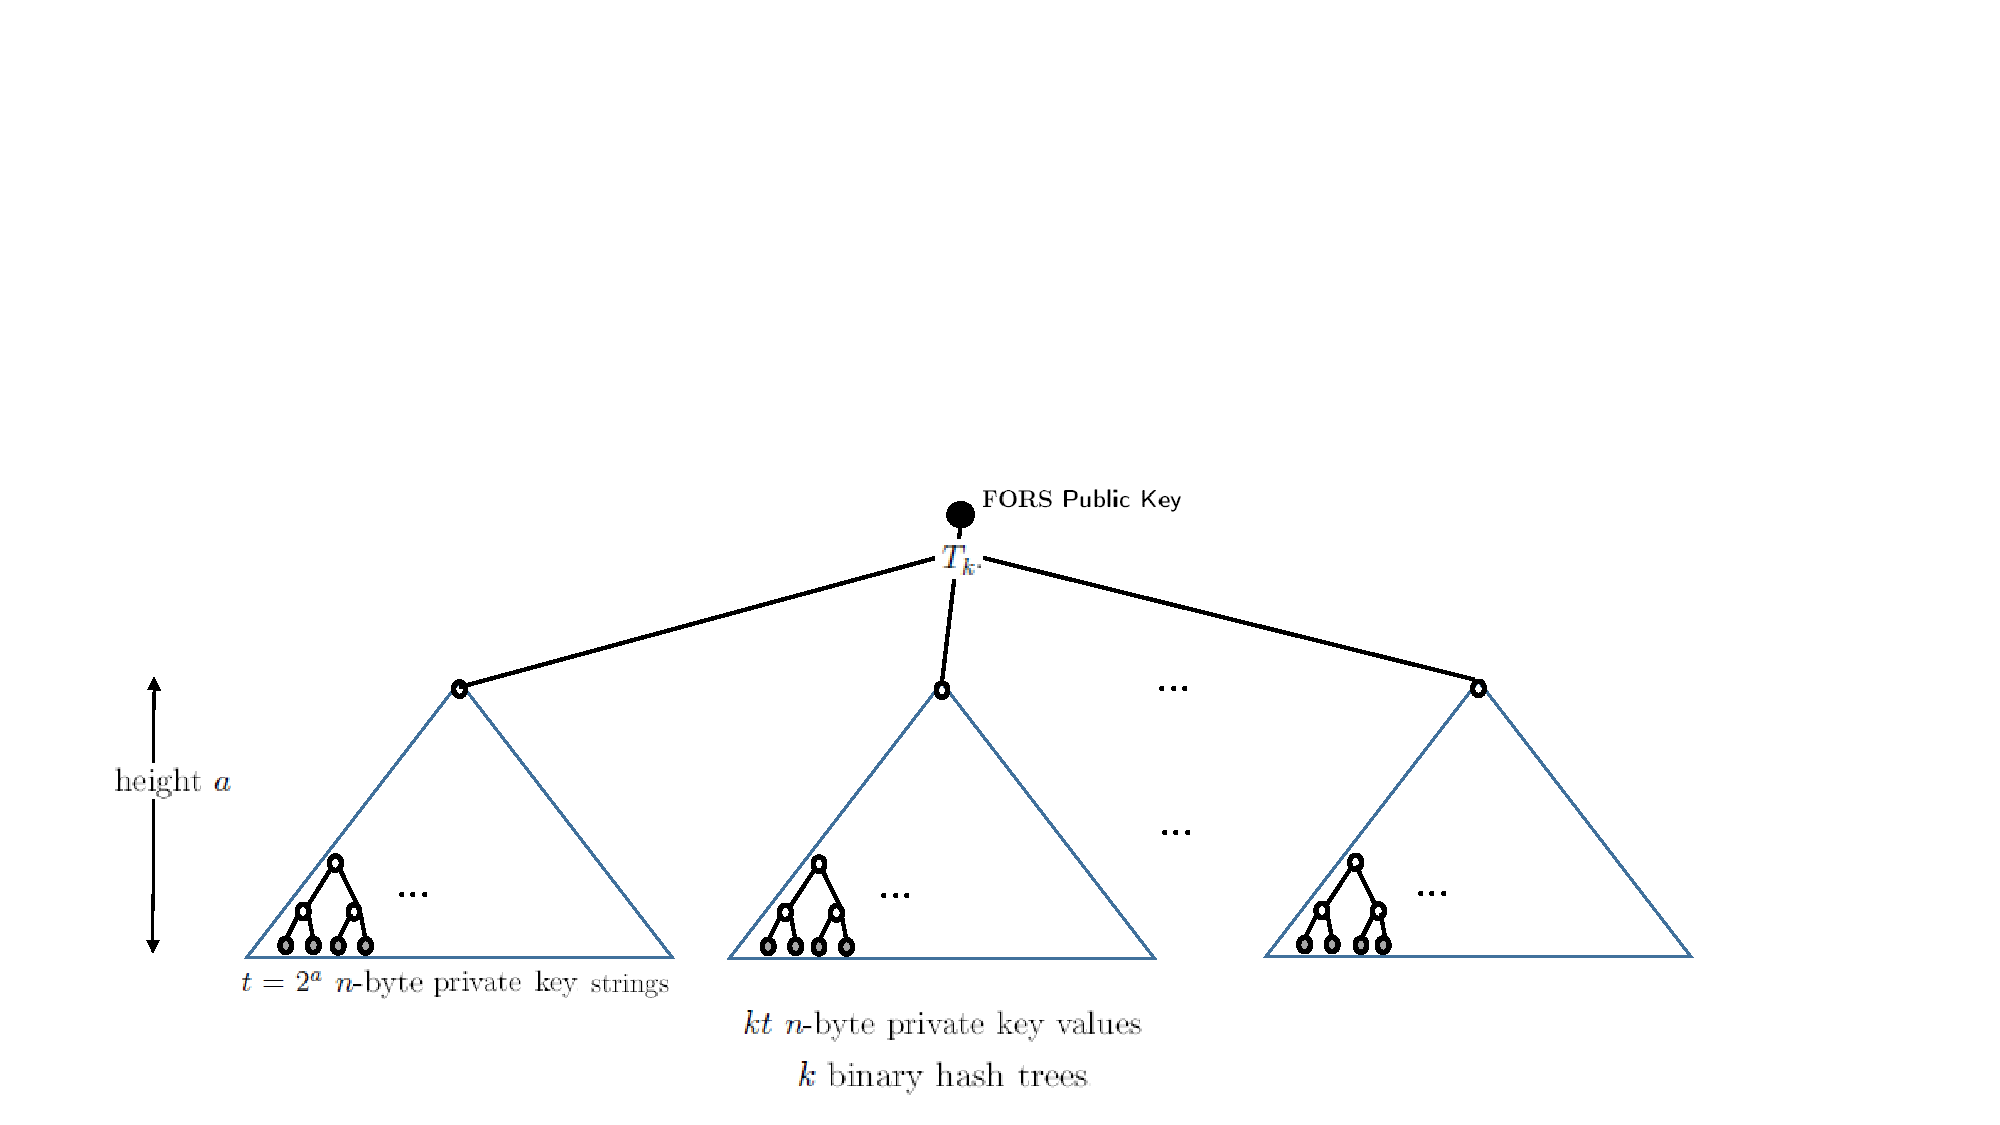
\includegraphics[width=7in,trim={0.5cm 0.5cm 0.5cm 7cm}, clip]{pics/fors_tree.pdf}
\caption{FORS trees and PK}
\end{figure}

\subsection{\fors Private Key (Function \texttt{fors\_SKgen})} 
In the context of \spx, a \fors private key is the single private seed \sseed
contained in the \spx private key. It is used to generate the $kt$ $n$-byte 
private key values using \sphincsPRF with a \fors key generation address. While these values are 
logically grouped into a two-dimensional array, for implementations it makes sense to assume they 
are in a one-dimensional array of length $kt$. 
The $j$th element of the $i$th set is then stored at $\sk[it + j]$. 
\begin{code}
  fors_SKgen' : ([n]Byte, Address) -> FORSPrKey
  fors_SKgen'(SKseed, ADRS) =
    [(fors_SKgen(SKseed, ADRS, i*`t+j)) | j <- [0 .. t-1], i <- [0 .. k-1]]
\end{code}
To generate one of these elements, a \fors key generation address \skadrs is used, that encodes the 
position of the \fors key pair within \spx and has 
tree height set to $0$ and leaf index set to $it+j$: 

\begin{lstlisting}[label=alg:fors_skgen, language=pseudoc,
                   caption=\texttt{fors\_SKgen} -- Computing a \fors private key value.]
#Input: secret seed SK.seed, address ADRS, secret key index idx = it+j
#Output: FORS private key sk

fors_SKgen(SK.seed, ADRS, idx) {
  skADRS = ADRS; // copy address to create key generation address
  skADRS.setType(FORS_PRF);
  skADRS.setKeyPairAddress(ADRS.getKeyPairAddress());
  
  skADRS.setTreeHeight(0);
  skADRS.setTreeIndex(idx);
  sk = PRF(SK.seed, skADRS);

  return sk;
}
\end{lstlisting}

\begin{code}
  fors_SKgen : ([n]Byte, Address, Integer) -> [n]Byte
  fors_SKgen(SKseed, ADRS, idx) = sk where
    skADRS0 = ADRS // copy address to create key generation address
    skADRS1 = setType(skADRS0, FORS_PRF)
    skADRS2 = setKeyPairAddress(skADRS1, getKeyPairAddress(ADRS))

    skADRS3 = setTreeHeight(skADRS2, 0)
    skADRS4 = setTreeIndex(skADRS3, idx)
    sk = PRF(SKseed, skADRS4)
\end{code}

\subsection{\fors TreeHash (Function \forstreehash)}
   Before coming to the \fors public key, we have to discuss computation of the 
   trees.
   For the computation of the $n$-byte nodes in the \fors hash trees,
   the subroutine \forstreehash is used. It is essentially the same algorithm
   as \treehash (\autoref{algo:treehash}) in \autoref{sec:xmss}. The two 
   differences are how the leaf nodes are computed and how addresses are handled.
   However, as the addresses are similar, an implementation can implement both
   algorithms in the same routine easily.
   
   Algorithm \forstreehash accepts a secret seed \sseed,
   a public seed \pseed, an unsigned integer $s$ (the start index), an
   unsigned integer $z$ (the target node height), and an address \adrs that
   encodes the address of the \fors key pair. As for \treehash, the
   \forstreehash algorithm returns the root node of a tree of height $z$ with
   the leftmost leaf being the hash of the private key element at index $s$. 
   Here, $s$ is ranging over the whole $kt$ private key elements.
   It is REQUIRED that $s\ \%\ 2^z = 0$, i.e. that the leaf at index $s$ is a
   leftmost leaf of a sub-tree of height $z$.  Otherwise the algorithm fails
   as it would compute non-existent nodes.  
   
   \begin{lstlisting}[breaklines=true, label=algo:forstreehash, language=pseudoc,
                   caption=The \forstreehash algorithm.]

# Input: Secret seed SK.seed, start index s, target node height z, public seed PK.seed, address ADRS
# Output: n-byte root node - top node on Stack

fors_treehash(SK.seed, s, z, PK.seed, ADRS) {
     if( s % (1 << z) != 0 ) return -1;
     for ( i = 0; i < 2^z; i++ ) {
       sk = fors_SKgen(SK.seed, ADRS, s+i) 
       node = F(PK.seed, ADRS, sk);
       ADRS.setTreeHeight(1);
       ADRS.setTreeIndex(s + i);
       while ( Top node on Stack has same height as node ) {
          ADRS.setTreeIndex((ADRS.getTreeIndex() - 1) / 2);
          node = H(PK.seed, ADRS, (Stack.pop() || node));
          ADRS.setTreeHeight(ADRS.getTreeHeight() + 1);
       }
       Stack.push(node);
     }
     return Stack.pop();
}

\end{lstlisting}

\begin{code}
  // We define fors_treehash recursively
  fors_treehash : ([n]Byte, [32], Integer, [n]Byte, Address) -> [n]Byte
  fors_treehash(SKseed, s, z, PKseed, ADRS) =
    if z == 0 then
    // leaf case
      F(PKseed, ADRS', (PRF(SKseed, ADRS')))
    else
      // internal node case
      H(PKseed, ADRS', hashL # hashR)
    where
      ADRS' = setTreeHeight((setTreeIndex(ADRS, toInteger(s >> z))), z)
      z' = z - 1
      hashL = fors_treehash(SKseed, s, z', PKseed, ADRS)
      hashR = fors_treehash(SKseed, (s + (1<<z')), z', PKseed, ADRS)
\end{code}

\subsection{\fors Public Key (Function \forspkgen)}
In the context of \spx, the \fors public key is never generated alone. It is 
only generated together with a signature. We include \forspkgen
for completeness, a better understanding, and testing. Algorithm \forspkgen takes 
a private seed \sseed, a public seed \pseed, and a \fors address \adrs. The 
latter encodes the position of the \fors instance within \spx. It outputs a 
\fors public key.

\begin{lstlisting}[label=alg:fors:pkgen, language=pseudoc,
                   caption=\forspkgen\ -- Generate a FORS public key.]

# Input: Secret seed SK.seed, public seed PK.seed, address ADRS
# Output: FORS public key PK

fors_PKgen(SK.seed, PK.seed, ADRS) {
     forspkADRS = ADRS; // copy address to create FTS public key address

     for(i = 0; i < k; i++){
         root[i] = fors_treehash(SK.seed, i*t, a, PK.seed, ADRS);
     }
     forspkADRS.setType(FORS_ROOTS);
     forspkADRS.setKeyPairAddress(ADRS.getKeyPairAddress());
     pk = T_k(PK.seed, forspkADRS, root);
     return pk;
}
\end{lstlisting}

\begin{code}
  fors_PKgen : ([n]Byte, [n]Byte, Address) -> FORSPbKey
  fors_PKgen(SKseed, PKseed, ADRS) = pk where
    forspkADRS = ADRS // copy address to create FTS public key address

    root = [fors_treehash(SKseed, fromInteger(i*`t), `a, PKseed, ADRS)
            | i <- [0 .. k-1]]
    forspkADRS' = setType(forspkADRS, FORS_ROOTS)
    forspkADRS'' = setKeyPairAddress(forspkADRS', getKeyPairAddress(ADRS))
    pk = T`{k}(PKseed, forspkADRS'', join root)
\end{code}

\subsection{\fors Signature Generation (Function \forssign)}
A \fors signature is a length $k(\log t + 1)$ array of $n$-byte strings. It contains 
$k$ private key values, $n$-bytes each, and their associated authentication
paths, $\log t$ $n$-byte values each.

\begin{code}
  // the spec concatenates everything so we consider an array of bytes
  // instead of an array of n-bytes.
  type FORSSig = [k*(logt+1)*n]Byte
\end{code}

The algorithm \forssign takes a $(k\log t)$-bit string $M$, a private seed \sseed, 
a public seed \pseed, and an address \adrs. The latter encodes the position of 
the \fors instance within \spx. It outputs a \fors signature \forssig.

\begin{lstlisting}[label=alg:fors_sign, language=pseudoc,
                   caption=\forssign\ -- Generating a FORS signature on string $M$.]
#Input: Bit string M, secret seed SK.seed, address ADRS, public seed PK.seed
#Output: FORS signature SIG_FORS

fors_sign(M, SK.seed, PK.seed, ADRS) {  
  // compute signature elements 
  for(i = 0; i < k; i++){
    // get next index
    unsigned int idx = bits i*log(t) to (i+1)*log(t) - 1 of M;
    
    // pick private key element
    SIG_FORS = SIG_FORS || fors_SKgen(SK.seed, ADRS, i*t + idx) ;
    
    // compute auth path
    for ( j = 0; j < a; j++ ) {
      s = floor(idx / (2^j)) XOR 1;
      AUTH[j] = fors_treehash(SK.seed, i * t + s * 2^j, j, PK.seed, ADRS);
    } 
    SIG_FORS = SIG_FORS || AUTH;
  }
  return SIG_FORS;
}
\end{lstlisting}

\begin{code}
  fors_sign : (FORSMessage, [n]Byte, [n]Byte, Address) -> FORSSig
  fors_sign(M, SKseed, PKseed, ADRS) = SIG_FORS where
    mkSIG i = SIG_FORSi # AUTHi where
      // get next index
      idx = toInteger ((groupBy`{logt} M)@i)

      // pick private key element
      SIG_FORSi = fors_SKgen(SKseed, ADRS, i*`t + idx) : [n]Byte

      // compute auth path
      AUTHi = join [mkAUTH j | j <- [0 .. a-1]] : [logt*n]Byte
      mkAUTH j = AUTHj where
        s = toInteger(fromInteger`{[a]}(floor(ratio idx 2^^j)) ^ 1)
        AUTHj =
          fors_treehash(SKseed, fromInteger(i*`t + s*2^^j), j, PKseed, ADRS)

    SIG_FORS = join [mkSIG i | i <- [0 .. k-1]]
\end{code}

The data format for a signature is given in \autoref{fig:fors:sig}.

\begin{figure} [h]
  \begin{center}
    \begin{tabular}{|c|}
      \hline
      \\[-0.5em] Private key value (tree 0) ($n$ bytes) \\[-0.5em] \\ \hline
      \\[-0.5em] \auth (tree 0) ($\log t\cdot n$ bytes) \\[-0.5em] \\ \hline
      \\[-0.5em] ... \\[-0.5em] \\ \hline
      \\[-0.5em] Private key value (tree $k-1$) ($n$ bytes) \\[-0.5em] \\ \hline
      \\[-0.5em] \auth (tree $k-1$) ($\log t\cdot n$ bytes) \\[-0.5em] \\ \hline
    \end{tabular}
  \end{center}
  \caption{\fors signature}
  \label{fig:fors:sig}
\end{figure}

\subsection{\fors Compute Public Key from Signature (Function \forspkfromsig)}

   \spx makes use of implicit signature verification of \fors signatures. 
   A \fors signature is used to compute a candidate \fors public key. This 
   public key is used in further computations (message for the signature of 
   the \xmss tree above) and implicitly verified by the outcome of that computation. Hence, this specification does 
   not contain a \texttt{fors\_verify} method but the method 
   \forspkfromsig. 
   
   The method \forspkfromsig takes a $k\log t$-bit string \msg, 
   a \fors signature \forssig, a public seed \pseed, and 
   an address \adrs. The latter encodes the position of the \fors 
   instance within the virtual structure of the \spx key pair. 
   First, the roots of the $k$ binary hash trees are computed using 
   \forstreehash. Afterwards the roots are hashed using the tweakable hash
   function $\sphincsT_k$.
%    \TODO {Clarify that this step takes place by the signer. --Andy: No, it takes place at signer AND verifier. On the signer side it is kind of a misuse of this method.}
   The algorithm \forspkfromsig is given 
   as \autoref{alg:fors:rootFromSig}. The method \forspkfromsig makes use of 
   functions $\forssig\texttt{.getSK(i)}$ and $\forssig\texttt{.getAUTH(i)}$. The 
   former returns the $i$th secret key element stored in the 
   signature, the latter returns the $i$th authentication path stored in
   the signature.
%    \TODO{Looks like what is missing here is that you calculate the FORS PK and compare it to the 
%    PK extracted with \forspkfromsig. --Andy: No, that's exactly what implicit signature verification is about. }

\begin{code}
  getSK : (FORSSig, Integer) -> [n]Byte
  getSK(SIG_FORS, i) = take`{n}((split`{k}SIG_FORS)@i)

  getAUTH : (FORSSig, Integer) -> [logt][n]Byte
  getAUTH(SIG_FORS, i) = groupBy(drop`{n}((split`{k}SIG_FORS)@i))
\end{code}
   
   
\begin{lstlisting}[breaklines=true, label=alg:fors:rootFromSig, language=pseudoc,
                   caption=\forspkfromsig\ -- 
                   Compute a \fors public key from a \fors signature.]

# Input: FORS signature SIG_FORS, (k lg t)-bit string M, public seed PK.seed, address ADRS
# Output: FORS public key

fors_pkFromSig(SIG_FORS, M, PK.seed, ADRS){
     
  // compute roots
  for(i = 0; i < k; i++){
    // get next index
    unsigned int idx = bits i*log(t) to (i+1)*log(t) - 1 of M;
    
    // compute leaf
    sk = SIG_FORS.getSK(i);
    ADRS.setTreeHeight(0);
    ADRS.setTreeIndex(i*t + idx);
    node[0] = F(PK.seed, ADRS, sk);
     
    // compute root from leaf and AUTH
    auth = SIG_FORS.getAUTH(i);
    ADRS.setTreeIndex(i*t + idx);
    for ( j = 0; j < a; j++ ) {
      ADRS.setTreeHeight(j+1);
      if ( (floor(idx / (2^j)) % 2) == 0 ) {
        ADRS.setTreeIndex(ADRS.getTreeIndex() / 2);
        node[1] = H(PK.seed, ADRS, (node[0] || auth[j]));
      } else {
        ADRS.setTreeIndex((ADRS.getTreeIndex() - 1) / 2);
        node[1] = H(PK.seed, ADRS, (auth[j] || node[0]));
      }
      node[0] = node[1];
    }
    root[i] = node[0];
  }

  forspkADRS = ADRS; // copy address to create FTS public key address
  forspkADRS.setType(FORS_ROOTS);
  forspkADRS.setKeyPairAddress(ADRS.getKeyPairAddress());
  pk = T_k(PK.seed, forspkADRS, root);
  return pk;
}
\end{lstlisting}

\begin{code}
  fors_pkFromSig : (FORSSig, FORSMessage, [n]Byte, Address) -> FORSPbKey
  fors_pkFromSig(SIG_FORS, M, PKseed, ADRS) = pk where

    //compute roots
    root = join [compRoots i| i<-[0 .. k-1]] : [k*n]Byte
    compRoots i = rooti where

      //get next index
      idx = toInteger ((groupBy`{logt} M)@i)

      // compute leaf
      sk = getSK(SIG_FORS, i)
      ADRSi = setTreeHeight(ADRS, 0)
      ADRSi' = setTreeIndex(ADRSi, i*`t + idx)
      node0 = F(PKseed, ADRSi', sk)

      //compute root from leaf and AUTH
      auth = getAUTH(SIG_FORS, i)
      ADRSi'' = setTreeIndex(ADRSi', i*`t + idx) //redundant

      rooti = foldl computeNode node0 [0 .. a-1]

      computeNode prevnode j = nextnode where 
        ADRSj = setTreeHeight(ADRSi'', j+1)
        nextnode =
          if ( (floor(ratio idx 2^^j) % 2) == 0 ) then
            H(PKseed, ADRSj', (prevnode # (auth@j))) where
              ADRSj' = setTreeIndex(ADRSj, getTreeIndex(ADRSj) / 2)
          else
            H(PKseed, ADRSj'', (auth@j)#prevnode) where
              ADRSj'' = setTreeIndex(ADRSj, (getTreeIndex(ADRSj) - 1) / 2)

    forspkADRS = ADRS // copy address to create FTS public key address
    forspkADRS' = setType(forspkADRS, FORS_ROOTS)
    forspkADRS'' = setKeyPairAddress(forspkADRS', getKeyPairAddress(ADRS))
    pk = T`{k}(PKseed, forspkADRS'', root)
\end{code}

\section{\spx}
%\section{The \spx Construction}
\label{sec:spx}
We now have all ingredients to describe our main construction \spx. 
Essentially, \spx is an orchestration of the methods and schemes described 
before. It only adds randomized message compression and verifiable index
generation. 

\subsection{\spx Parameters}

\spx has the following parameters:
\begin{description}
 \item  $n$ : the security parameter in bytes.
 \item  $w$ : the Winternitz parameter as defined in \autoref{sec:wots:params}.
 \item  $h$ : the height of the hypertree as defined in \autoref{sec:ht:params}.
 \item  $d$ : the number of layers in the hypertree as defined in \autoref{sec:ht:params}.
 \item  $k$ : the number of trees in \fors as defined in \autoref{sec:fors:params}.
 \item  $t$ : the number of leaves of a \fors tree as defined in \autoref{sec:fors:params}.
\end{description}

\begin{code}
  parameter
    type h : #
    type constraint (fin h)
    type d : #
    type constraint (d >= 2, h%d == 0, h/d >= 1)
    // the following constraint is needed because
    // h - h/d bits should define a tree address
    type constraint (3*4*8 >= h - h/d)
    type k : #
    type constraint (fin k, k >= 1)
    // instead of t, we consider a = log t as the parameter since
    // it is a that is instantiated.
    type a : #
    type constraint (fin a, a >= 1)

  type t = 2^^a
  type logt = a
\end{code}

All the restrictions stated in the previous sections apply. Recall that 
we use $a = \log t$. Moreover, from these values the values $m$ and \len are
computed as
\begin{itemize}
  \item $m$: the message digest length in bytes. 
  It is computed as 
  $$m=\floor{(k\log t +7)/ 8} + \floor{(h - h/d +7)/ 8} + \floor{(h / d +7)/ 8}.$$

\begin{code}
  type m = (k*logt+7)/8 + (h-h/d+7)/8 + (h/d+7)/8
\end{code}

  While only $h + k\log t$ bits would be needed, using the longer $m$ as defined 
  above simplifies implementations significantly.
  \item $\len$: the number of $n$-byte string elements in a \wotsp private
        key, public key, and signature. It is computed as $\len =
        \len_1 + \len_2$, with
        \begin{equation*}
          \len_1 = \ceil*{\frac{8n}{\log(w)}},\
          \len_2 = \floor*{\frac{\log{(\len_1(w - 1))}}{\log(w)}} + 1
        \end{equation*}

\begin{code}
  // len, len1 and len2 have been defined earlier
\end{code}
\end{itemize}

In the following, we assume that all algorithms have access to these parameters.

\subsection{\spx Key Generation (Function \spxkgen)}

   The \spx private key contains two elements. First, the $n$-byte secret seed 
   \sseed which is used to generate all the \wotsp and \fors private key elements. 
   Second, an $n$-byte PRF key \skprf which is used to deterministically 
   generate a randomization value for the randomized message hash. 

   The \spx public key also contains two elements. First, the \hyper public key, 
   i.e. the root of the tree on the top layer. Second, an $n$-byte public seed
   value \pseed which is sampled uniformly at random.
   
   As \spxsign does not get the public key, but needs access to \pseed (and 
   possibly to \proot for fault attack mitigation), the \spx secret key contains 
   a copy of the public key.

\begin{code}
  type SK_SPHINCS = ([n]Byte, [n]Byte, [n]Byte, [n]Byte)
  type PK_SPHINCS = ([n]Byte, [n]Byte) 
\end{code}
   
   The description of algorithm \spxkgen assumes the existence of a function 
   \texttt{sec\_rand} which on input $i$ returns $i$-bytes of cryptographically strong
   randomness.

\begin{lstlisting}[label=alg:spx:pkgen, language=pseudoc,
                   caption=\spxkgen\ -- Generate a \spx key pair.]

# Input: (none)
# Output: SPHINCS+ key pair (SK,PK)

spx_keygen( ){          
     SK.seed = sec_rand(n);
     SK.prf = sec_rand(n);
     PK.seed = sec_rand(n);
     PK.root = ht_PKgen(SK.seed, PK.seed);
     return ( (SK.seed, SK.prf, PK.seed, PK.root), (PK.seed, PK.root) );
}

\end{lstlisting}

\begin{code}
  spx_keygen : ([n]Byte, [n]Byte, [n]Byte) -> (SK_SPHINCS, PK_SPHINCS)
  spx_keygen(SKseed, SKprf, PKseed) =
    ( (SKseed, SKprf, PKseed, PKroot), (PKseed, PKroot) )
    where 
      PKroot = ht_PKgen(SKseed, PKseed)
\end{code}

    The format of a \spx private and public key is given in \autoref{fig:spx:keys}.

\begin{figure} [h]
  \begin{center}
  \begin{minipage}{.4\textwidth}
        \begin{center}
	  \begin{tabular}{|c|}
	    \hline
	    \\[-0.5em] \sseed ($n$ bytes) \\[-0.5em] \\ \hline
	    \\[-0.5em] \skprf ($n$ bytes) \\[-0.5em] \\ \hline
	    \\[-0.5em] \pseed ($n$ bytes) \\[-0.5em] \\ \hline
	    \\[-0.5em] \proot ($n$ bytes) \\[-0.5em] \\ \hline
	  \end{tabular}
        \end{center}
      \end{minipage}
  \begin{minipage}{.4\textwidth}
      \begin{center}
	\begin{tabular}{|c|}
	    \hline
	    \\[-0.5em] \pseed ($n$ bytes) \\[-0.5em] \\ \hline
	    \\[-0.5em] \proot ($n$ bytes) \\[-0.5em] \\ \hline
	  \end{tabular}
        \end{center}
      \end{minipage}
  \end{center}
  \caption{Left: \spx secret key. Right: \spx public key.} 
  \label{fig:spx:keys}
\end{figure}

\subsection{\spx Signature}

   A \spx signature \htsig is a byte string of length $(1 + k(a + 1) + h + d\len)n$.  
   It consists of an $n$-byte randomization string $R$, a \fors signature 
   \forssig consisting of $k(a+1)$ $n$-byte strings, and a \hyper signature \htsig 
   of $(h + d\len)n$ bytes.

\begin{code}
  type SIG_SPHINCS = [(1 + k*(a+1) + h + d*len) * n]Byte
\end{code}

   The data format for a signature is given in \autoref{fig:xmssmt:sig}

%Not so elegant way for the table in the figure below with the right row height.
\begin{figure} [h]
  \begin{center}
    \begin{tabular}{|c|}
      \hline
      \\[-0.5em] Randomness \Random ($n$ bytes) \\[-0.5em] \\ \hline
      \\[-0.5em] \fors signature \forssig ($k(a+1) \cdot n$ bytes) \\[-0.5em] \\ \hline
      \\[-0.5em] \hyper signature \htsig ($(h +d\len)n$ bytes) \\[-0.5em] \\ \hline
    \end{tabular}
  \end{center}
  \caption{\spx signature} 
  \label{fig:spx:sig}
\end{figure}

\subsection{\spx Signature Generation (Function \spxsign)}
   Generating a \spx signature consists of four steps. First, a random value 
   \Random
   is pseudorandomly generated. Next, this is used to compute a $m$ byte message 
   digest which is split into a $\floor{(k\log t +7)/ 8}$-byte partial message
   digest $\texttt{tmp\_md}$, a $\floor{(h - h/d +7)/ 8}$-byte tree index $\texttt{tmp\_idx\_tree}$, and 
   a $\floor{(h / d +7)/ 8}$-byte 
   leaf index $\texttt{tmp\_idx\_leaf}$. Next, the actual values \md,
   $\texttt{idx\_tree}$, and $\texttt{idx\_leaf}$ are computed by extracting the 
   necessary number of bits.
   The partial message digest
   \md is then signed with the $\texttt{idx\_leaf}$-th 
   \fors key pair of the $\texttt{idx\_tree}$-th \xmss tree on the lowest \hyper layer. 
   The public key of the \fors key pair is then signed using 
   \hyper. As described in Section~\ref{sec:hyper:sign}, the index is never
   actually used as a whole, but immediately split into a tree index
   and a leaf index, for ease of implementation.
   
   When computing \Random, the PRF takes a $n$-byte string \texttt{opt} 
   which is initialized with \pseed but can be overwritten with randomness
   if the global variable RANDOMIZE is set. This option is given as otherwise
   \spx signatures would be always deterministic. This might be problematic in 
   some settings. See \autoref{sec:security} and \autoref{sec:discussion} for 
   more details.

\begin{lstlisting}[label=alg:spx:sign, mathescape, language=pseudoc,
                   caption=\spxsign\ -- Generating a \spx signature]
   
# Input: Message M, private key SK = (SK.seed, SK.prf, PK.seed, PK.root)
# Output: SPHINCS+ signature SIG

spx_sign(M, SK){
     // init
     ADRS = toByte(0, 32);
     
     // generate randomizer
     opt = PK.seed;
     if(RANDOMIZE){
       opt = rand(n);
     }
     R = PRF_msg(SK.prf, opt, M);
     SIG = SIG || R;
     
     // compute message digest and index
     digest = H_msg(R, PK.seed, PK.root, M);
     tmp_md = first floor((ka +7)/ 8) bytes of digest;
     tmp_idx_tree = next floor((h - h/d +7)/ 8) bytes of digest;
     tmp_idx_leaf = next floor((h/d +7)/ 8) bytes of digest;
     
     md = first ka bits of tmp_md;
     idx_tree = first h - h/d bits of tmp_idx_tree;
     idx_leaf = first h/d bits of tmp_idx_leaf;

     // FORS sign
     ADRS.setLayerAddress(0);
     ADRS.setTreeAddress(idx_tree);
     ADRS.setType(FORS_TREE);
     ADRS.setKeyPairAddress(idx_leaf);

     SIG_FORS = fors_sign(md, SK.seed, PK.seed, ADRS);
     SIG = SIG || SIG_FORS;
     
     // get FORS public key
     PK_FORS = fors_pkFromSig(SIG_FORS, md, PK.seed, ADRS);
     
     // sign FORS public key with HT
     ADRS.setType(TREE);
     SIG_HT = ht_sign(PK_FORS, SK.seed, PK.seed, idx_tree, idx_leaf);
     SIG = SIG || SIG_HT;
     
     return SIG;
}
\end{lstlisting}

\begin{code}
  spx_sign : {lmsg} (fin lmsg) => ([lmsg]Byte, SK_SPHINCS) -> SIG_SPHINCS
  spx_sign(M, SK) = SIG where
    (SKseed, SKprf, PKseed, PKroot) = SK
    // init
    ADRS = toByte`{32} 0

    // generate randomizer
    opt = PKseed
    
    R = PRF_msg(SKprf, opt, M) : [n]Byte

    // compute message digest and index
    digest = H_msg(R, PKseed, PKroot, M)
    tmp_md =
      take`{(k*a +7)/ 8} digest
    tmp_idx_tree =
      take`{(h - h/d +7)/ 8}(drop`{(k*a +7)/ 8} digest)
    tmp_idx_leaf =
      take`{(h/d +7)/ 8}(drop`{(k*a +7)/ 8 + (h - h/d +7)/ 8} digest)

    md = take`{k*a}(join tmp_md)
    idx_tree =
      groupBy`{8} (zext (take`{h - h/d}(join tmp_idx_tree))) : TreeAddress
    idx_leaf = toInteger(take`{h/d}(join tmp_idx_leaf))

    // FORS sign
    ADRS1 = setLayerAddress(ADRS, 0)
    ADRS2 = setTreeAddress(ADRS1, idx_tree)
    ADRS3 = setType(ADRS2, FORS_TREE)
    ADRS4 = setKeyPairAddress(ADRS3, idx_leaf)

    SIG_FORS = fors_sign(md, SKseed, PKseed, ADRS): FORSSig

    // get FORS public key 
    PK_FORS = fors_pkFromSig(SIG_FORS, md, PKseed, ADRS)

    // sign FORS public key with HT
    ADRS5 = setType(ADRS4, TREE)
    SIG_HT = ht_sign(PK_FORS, SKseed, PKseed, idx_tree, idx_leaf) : SIGHT

    SIG = R # SIG_FORS # SIG_HT
\end{code}

\subsection{\spx Signature Verification (Function \spxverify)}

   \spx signature verification (\autoref{alg:spx:ver}) can be summarized as 
   recomputing message digest and index, computing a candidate \fors public key,
   and verifying the \hyper signature on that public key. Note that the \hyper
   signature verification will fail if the \fors public key is not matching the
   real one (with overwhelming probability). \spx signature verification takes 
   a message \msg, a signature \spxsig, and a \spx public key \PK.

\begin{code}
  // The following trivial functions are used. We make them explicit.
  getR : SIG_SPHINCS -> [n]Byte
  getR(SIG) = take SIG

  getSIG_FORS : SIG_SPHINCS -> FORSSig
  getSIG_FORS(SIG) = take (drop SIG : [(k*(a+1) + h + d*len)*n]Byte)

  getSIG_HT : SIG_SPHINCS -> SIGHT
  getSIG_HT(SIG) = drop SIG
\end{code}

\begin{lstlisting}[breaklines=true, label=alg:spx:ver, mathescape, language=pseudoc,
                   caption=\spxverify\ -- Verify a \spx signature \spxsig on a
   message \msg using a \spx public key \PK]
   
# Input: Message M, signature SIG, public key PK
# Output: Boolean

spx_verify(M, SIG, PK){
     // init
     ADRS = toByte(0, 32);
     R = SIG.getR();
     SIG_FORS = SIG.getSIG_FORS();
     SIG_HT = SIG.getSIG_HT();

     
     // compute message digest and index
     digest = H_msg(R, PK.seed, PK.root, M);
     tmp_md = first floor((ka +7)/ 8) bytes of digest;
     tmp_idx_tree = next floor((h - h/d +7)/ 8) bytes of digest;
     tmp_idx_leaf = next floor((h/d +7)/ 8) bytes of digest;
     
     md = first ka bits of tmp_md;
     idx_tree = first h - h/d bits of tmp_idx_tree;
     idx_leaf = first h/d bits of tmp_idx_leaf;

     // compute FORS public key
     ADRS.setLayerAddress(0);
     ADRS.setTreeAddress(idx_tree);
     ADRS.setType(FORS_TREE);
     ADRS.setKeyPairAddress(idx_leaf);
     
     PK_FORS = fors_pkFromSig(SIG_FORS, md, PK.seed, ADRS);
     
     // verify HT signature
     ADRS.setType(TREE);
     return ht_verify(PK_FORS, SIG_HT, PK.seed, idx_tree, idx_leaf, PK.root);
}
\end{lstlisting}

\begin{code}
  spx_verify : {lmsg} (fin lmsg) =>
    ([lmsg]Byte, SIG_SPHINCS, PK_SPHINCS) -> Bit 
  spx_verify(M, SIG, PK) =
    ht_verify(PK_FORS, SIG_HT, PKseed, idx_tree, idx_leaf, PKroot)
    where 
      (PKseed, PKroot) = PK

      // init
      ADRS = toByte`{32} 0
      R = getR(SIG)
      SIG_FORS = getSIG_FORS(SIG)
      SIG_HT = getSIG_HT(SIG)

      // compute message digest and index
      digest = H_msg(R, PKseed, PKroot, M)
      tmp_md =
        take`{(k*a +7)/ 8} digest
      tmp_idx_tree =
        take`{(h - h/d +7)/ 8}(drop`{(k*a +7)/ 8} digest)
      tmp_idx_leaf =
        take`{(h/d +7)/ 8}(drop`{(k*a +7)/ 8 + (h - h/d +7)/ 8} digest)

      md = take`{k*a}(join tmp_md)
      idx_tree =
        groupBy`{8} (zext (take`{h - h/d}(join tmp_idx_tree))) : TreeAddress
      idx_leaf = toInteger(take`{h/d}(join tmp_idx_leaf))

      // compute FORS public key
      ADRS1 = setLayerAddress(ADRS, 0)
      ADRS2 = setTreeAddress(ADRS1, idx_tree)
      ADRS3 = setType(ADRS2, FORS_TREE)
      ADRS4 = setKeyPairAddress(ADRS3, idx_leaf)

      PK_FORS = fors_pkFromSig(SIG_FORS, md, PKseed, ADRS)

      // verify HT signature
      ADRS5 = setType(ADRS4, TREE) // redundant
\end{code}

\begin{code}
  CorrectnessSPHINCSPlus : ([n]Byte, [n]Byte, [n]Byte) -> Bit
  property CorrectnessSPHINCSPlus(SKseed, SKprf, PKseed) = spx_verify`{10}(M, SIG, PK)
    where
      (SK, PK) = spx_keygen(SKseed, SKprf, PKseed)
      M = zero
      SIG = spx_sign`{10}(M, SK)
\end{code}

\section{Instantiations}
\label{sec:instantiations}

This section discusses instantiations for \spx. \spx can be 
viewed as a signature template. It is a way to build a signature 
scheme by instantiating the cryptographic function families used. We consider
different ways to implement the cryptographic function families as 
different signature systems. Orthogonal to instantiating the cryptographic 
function families are parameter sets. Parameter sets
assign  specific values to the \spx parameters described in \autoref{sec:spx:params} below. 

In this section, we first define the requirements on parameters and discuss 
existing trade-offs between 
security, sizes, and speed controlled by the different parameters. Then we 
propose 6 different parameter sets that match NIST security levels $I$, 
$III$, and $V$ (2 parameter sets per security level). Afterwards we propose 
three different instantiations for the cryptographic function families of \spx. 
These instantiation are indeed three different signature schemes. We propose 
\spx-\shathree, \spx-\shatwo, and \spx-\haraka. The 
former two use the cryptographic hash functions defined in FIPS PUB 202, 
respectively FIPS PUB 180, to instantiate the cryptographic function families. 
The latter uses a new cryptographic (hash) function called \haraka, proposed in
\cite{articleToSC563}. 

\subsection{\spx Parameter Sets}\label{sec:spx:params}
\spx is described by the following parameters already described in the previous 
sections. All parameters take positive integer values.
\begin{description}
 \item  $n$ : the security parameter in bytes.
 \item  $w$ : the Winternitz parameter.
 \item  $h$ : the height of the hypertree.
 \item  $d$ : the number of layers in the hypertree.
 \item  $k$ : the number of trees in \fors.
 \item  $t$ : the number of leaves of a \fors tree.
\end{description}

Recall that 
we use $a = \log t$. Moreover, from these values the values $m$ and \len are
computed as
\begin{itemize}
  \item $m$: the message digest length in bytes. 
  It is computed as $m = \floor{(k\log t +7)/ 8} + \floor{(h - h/d +7)/ 8} + \floor{(h / d +7)/ 8}$.
  \item $\len$: the number of $n$-byte string elements in a \wotsp private
        key, public key, and signature. It is computed as $\len =
        \len_1 + \len_2$, with
        \begin{equation*}
          \len_1 = \ceil*{\frac{8n}{\log(w)}},\
          \len_2 = \floor*{\frac{\log{(\len_1(w - 1))}}{\log(w)}} + 1
        \end{equation*}
\end{itemize}

We now repeat the roles of, requirements on, and properties of these parameters.
Afterwards, we give several formulas that show their exact influence on 
performance and security.

The security parameter $n$ is also the output length of all cryptographic function 
families besides \sphincsHmsg. Therefore, it largely determines which security 
level a parameter set reaches. It is also the size of virtually any node 
within the \spx structure and thereby also the size of all elements in a 
signature, i.e., the signature size is a multiple of $n$. 

The Winternitz parameter $w$ determines the number and length of the hash chains per 
\wotsp instance. A greater value for $w$ linearly increases the length of the 
hash chains but logarithmically reduces their number. The number of hash 
chains exactly corresponds to the number of $n$-byte values in a \wotsp 
signature. Thereby it largely influences the size of a \spx signature. 
The product of the number and the length of hash chains directly correlates with 
signing speed as essentially all time in \hyper signature generation is spent 
computing \wotsp public keys. Therefore, greater $w$ means shorter signatures 
but slower signing. However, note the exponential gap. The bigger $w$ gets, 
the more expensive is the signature size reduction. The Winternitz parameter 
does not influence \spx security.

The height of the hypertree $h$ determines the number of \fors instances. Hence,
it determines the probability that a \fors key pair is used several times, 
given the number of signatures made with a \spx key pair. Hence, the height has 
a direct impact on security: A taller hypertree gives more security. On the 
other hand, a taller tree leads to larger signatures.

The number of layers $d$ is a pure performance trade-off parameter and does not
influence security. It determines the number of layers of \xmss trees in the 
hypertree. Hence, $d$ must divide $h$ without remainder. The parameter $d$ 
thereby defines the height of the \xmss trees used. The greater $d$, the smaller
the subtrees, the faster signing. However, $d$ also controls the number of 
layers and thereby the number of \wotsp signatures within a \hyper and thereby 
a \spx signature. 

The parameters $k$ and $t$ determine the performance and security of \fors. The 
number of leaves of a tree in \fors $t$ must be a power of two while $k$ can be
chosen freely. A smaller $t$ generally leads to smaller and faster signatures.
However, for a given security level a smaller $t$ requires a greater $k$
which increases signature size and slows down signing. Hence, it is important 
to balance these two parameters. This is best done using the formulas below.

The message digest length $m$ is the output length of \sphincsHmsg in bytes. 
It is $\floor{(k\log t +7)/ 8} + \floor{(h - h/d +7)/ 8} + \floor{(h / d +7)/ 8}$ 
bytes. 

The number $\len$ of chains in a \wotsp key pair determines the \wotsp signature size.

\subsubsection{Influence of Parameters on Security and Performance}
\label{sec:generic-estimates}
In the following we provide formulas to compute speed, size and security for 
a given \spx parameter set. This supports parameter selection. We also provide
a SAGE script in \autoref{sec:evalscript}.

\paragraph{Key Generation.} Generating the \spx private key and \pseed requires 
three calls to a secure random number generator. Next we have to generate the 
top tree. For the leaves we need to do $2^{h/d}$ \wotsp key generations ($\len$ 
calls to \sphincsPRF for generating the \sk and $w \len$ calls to \sphincsF for the \pk) 
and we have to compress the \wotsp public key (one call to $T_\len$). Computing 
the root of the top tree requires $(2^{h/d} - 1)$ calls to \sphincsH.

\paragraph{Signing.} For randomization and message compression we need one call to
%$\sphincsPRF$, 
$\sphincsPRFmsg$, and one to $\sphincsHmsg$. The \fors signature requires 
$kt$ calls to \sphincsPRF and \sphincsF. Further, we have to compute the root of 
$k$ binary trees of height $\log t$ which adds $k(t - 1)$ calls to \sphincsH. 
Finally, we need one call to $T_k$. Next, we compute one HT signature which 
consists of $d$ trees similar to the key generation. Hence, we have to do 
$d(2^{h/d})$ times $\len$ calls to \sphincsPRF and $w\len$ calls to \sphincsF
as well as $d(2^{h/d})$ calls to $\sphincsT_\len$. For computing 
the root of each tree we get additionally $d(2^{h/d} - 1)$ calls to \sphincsH.

\paragraph{Verification.} First we need to compute the message hash using 
$\sphincsHmsg$. We need to do one \fors verification which requires
$k$ calls to %\sphincsPRF and 
\sphincsF (to compute the leaf nodes from the signature elements), $k\log t$ calls to \sphincsH (to compute the root nodes using the leaf nodes and the authentication paths), and one call
to $T_k$ for hashing the roots. Next, we have to verify $d$ \xmss signatures 
which takes $<w\len$ calls to \sphincsF and one call to $T_\len$ each for \wotsp
signature verification\footnote{It should be noted that the $w\len$ bound for calls to \sphincsF is a worst-case bound. This is a bound on the cost for \wots signature verification. Given that the messages are hash values which can assumed to be close to uniformly distributed, this value will be closer to the average-case bound $(w/2) \cdot \len$ in actual measurements.}. It also needs $dh/d$ calls to \sphincsH for the $d$ 
root computations.

\begin{table}
   \centering
   \caption{Overview of the number of function calls we require for each 
            operation. We omit the single calls to $\sphincsHmsg, \sphincsPRFmsg$, 
            and $\sphincsT_k$ for signing and single calls to $\sphincsHmsg$ 
            and $\sphincsT_k$ for verification as they are negligible when
            estimating speed.}
   \label{tab:perfcalls}
   \begin{tabular}{lcccc}
      \toprule
               & \sphincsF & \sphincsH & \sphincsPRF & $T_\len$\\
      \midrule
      Key Generation & $2^{h/d}w\len $ 
                     & $2^{h/d} - 1$ 
                     & $2^{h/d}\len$ 
                     & $2^{h/d}$\\
      Signing        & $kt + d(2^{h/d})w\len$ 
                     & $k(t - 1) + d(2^{h/d} - 1)$ 
                     & $kt + d(2^{h/d})\len$ % + 1$ 
                     & $d2^{h/d}$\\
      Verification   & $k + dw\len$ 
                     & $k\log t + h$
                     & -- %$kt$
                     & $d$ \\
      \bottomrule
   \end{tabular}
\end{table} 
~\\ 
The size of the \spx private and public keys along with the signature can be deduced from \autoref{sec:spx}
and is shown in Table~\ref{tab:sizes}.

\begin{table}
   \centering
   \caption{Key and signature sizes}
   \label{tab:sizes}
   \begin{tabular}{lccc}
      \toprule
               & SK & PK & Sig \\
      \midrule
      Size & $4n$ 
           & $2n$ 
           & $(h+k(\log t+1) +d\cdot len+1)n$ \\
      \bottomrule
   \end{tabular}
\end{table}

% \TODO{Put formulas for security here }
The classical security level, or bit security of \spx against generic attacks can be computed as
$$b = - \log\left(
\frac{1}{2^{8n}} + \sum_\gamma
  \left(1-\left(1-{1\over t}\right)^\gamma\right)^k
  {q\choose \gamma}
  \left(1-{1\over 2^h}\right)^{q-\gamma}
  {1\over 2^{h\gamma}}\right).
  $$

The quantum security level, or bit security of \spx against generic attacks can be computed as
$$b = - \frac{1}{2} \log\left(
\frac{1}{2^{8n}} + \sum_\gamma
  \left(1-\left(1-{1\over t}\right)^\gamma\right)^k
  {q\choose \gamma}
  \left(1-{1\over 2^h}\right)^{q-\gamma}
  {1\over 2^{h\gamma}}\right).
  $$
Here, we are neglecting the small constant factors inside the logarithm. For details see \autoref{sec:security}.  


\subsubsection{Proposed Parameter Sets and Security Levels}
As explained in the previous subsection,
even for a fixed security level the design of \spx supports many different
tradeoffs between signature size and speed. In Table~\ref{tab:params} we list
6 parameter sets that%
---together with the cycle counts given in Table~\ref{tab:runtime}---
illustrates how these tradeoffs can be used to obtain concrete parameter sets
optimizing for signature size and concrete parameter sets optimizing for speed.
Specifically, we propose parameter sets achieving security levels 1, 3, and 5;
for each of these security levels propose one size-optimized (ending on `s'
for ``small'') and one speed-optimized (ending on `f' for ``fast'') parameter
set. The parameter sets were obtained with the help of a Sage script that 
we list in \autoref{sec:evalscript}. In the first line of that script,
set the ``target bit security'' to a desired value (in our case, close to
$128$ for security level 1, close to $192$ for security level 3, and close to $256$
for security level 5). The output of the script will be a long list of possible
parameters achieving this security level together with the signature size and
an estimate of the performance, using the formulas from 
\autoref{sec:generic-estimates} above.

Note that we did \emph{not} obtain our proposed parameter sets simply by searching
this output for the smallest or the fastest option. The reason is that, for example,
optimizing for size without caring about speed at all results in signatures of 
a size of $\approx15$\,KB for a bit security of $256$, but computing one signature
takes more than 20 minutes on our benchmark platform. Such a tradeoff might be
interesting for very few select applications, but we cannot think of many applications
that would accept such a large time for signing. Instead, the proposed parameter
sets are what we consider ``non-extreme''; i.e., with a signing time of at most
a few seconds in our non-optimized implementation.

The choice of these parameters is orthogonal to the choice of hash function.
In~\autoref{subsec:instanthash} we describe three different instantiations
of the underlying hash function, each with a simple and a robust variant.
Together with the six parameter sets listed in 
Table~\ref{tab:params} we obtain 36 different instantiations of \spx.

\begin{table}
  \caption{Example parameter sets for \spx targeting different security levels and different tradeoffs between size and speed. Note that these parameter sets have been update for round 3.
  The column labeled ``bitsec'' gives the bit security computed as described in~\autoref{sec:security}; 
  the column labeled ``sec level'' gives the security level according to the levels specified in Section 4.A.5 of the Call for Proposals.
  As explained later,
  \textbf{for Haraka the security level is limited to 2:}
  i.e., it is 1 for $n=16$, and 2 for $n=24$ or $n=32$.}
  \label{tab:params}
  \def\arraystretch{1.2}
  \begin{tabularx}{\textwidth}{Xrrrrrrrrr}
    \hline
                  & $n$  & $h$  & $d$  & $\log(t)$ & $k$  & $w$  & bitsec & sec level   & sig bytes \\
    \hline
    \spxlowsmall  & $16$ & $63$ &  $7$ &      $12$ & $14$ & $16$ &  $133$ %~=-log(1/128+1/133)/log2
	              & \textbf{1}  &  $7\,856$ \\
    \spxlowfast   & $16$ & $66$ & $22$ &       $6$ & $33$ & $16$ &  $128$ %=-log(1/128+1/128)/log2 
	              & \textbf{1}  & $17\,088$ \\
    \spxmidsmall  & $24$ & $63$ &  $7$ &      $14$ & $17$ & $16$ &  $193$ %~=-log(1/192+1/196)/log2
	              & \textbf{3}  & $16\,224$ \\
    \spxmidfast   & $24$ & $66$ & $22$ &       $8$ & $33$ & $16$ &  $194$ %~=-log(1/192+1/194)/log2
	              & \textbf{3}  & $35\,664$ \\
    \spxhighsmall & $32$ & $64$ &  $8$ &      $14$ & $22$ & $16$ &  $255$ %~=-log(1/256+1/255)/log2
	              & \textbf{5}  & $29\,792$ \\
    \spxhighfast  & $32$ & $68$ & $17$ &      $9$ & $35$ & $16$ &  $255$ %~=-log(1/256+1/254)/log2
	              & \textbf{5}  & $49\,856$ \\
    \hline
  \end{tabularx}
\end{table}


\subsection{Instantiations of Hash Functions}
\label{subsec:instanthash}
In this section we define different signature schemes, which are obtained 
by instantiating the cryptographic function families of \spx with \shatwo, 
\shathree, and \haraka. To instantiate the tweakable hash functions,
we present two different constructions. Leading to a total of six instantiations.
For the `robust' instances,
we first generate pseudorandom \emph{bitmasks}
which are then XORed with the input message. The masked messages are denoted
as $M^{\oplus}$.
For the `simple' instances, we take an approach inspired by the LMS proposal for stateful hash-based signatures~\cite{LMSdraft}, and omit the bitmasks.
We make this difference explicit in the instances defined below. The 'simple' instances 
are faster as they omit the calls to the underlying hash function to generate bitmasks. When combined with compressed addresses in the \shatwo case this can lead to an estimated reduction of the number of 
compression function calls by a factor of almost 4. In return, this comes at the cost of a 
security argument that entirely relies on the random oracle model. 

Recall that $n$ and $m$ are the security parameter and the message digest length, in bytes.

\subsubsection{\spx-\shathree}
   For \spx-\shathree we define
   \begin{equation}
      \begin{aligned}
         \sphincsHmsg(\Random,\pseed, \proot, M) &= \shaketfs(\Random || \pseed || \proot || M, 8m),\\
         \sphincsPRF(\pseed, \sseed, \adrs) &= \shaketfs(\pseed || \adrs || \sseed, 8n),\\
         \sphincsPRFmsg(\skprf, \texttt{OptRand}, M) &= \shaketfs(\skprf || \texttt{OptRand} || M, 8n).\\
      \end{aligned}
    \end{equation}

\begin{code}
  // Spec has a typo. PRF takes 2 parameters.
\end{code}

    For the robust variant, we further define the tweakable hash functions as
    \begin{equation}
      \begin{aligned}
         \sphincsF(\pseed, \adrs, M_1) &= \shaketfs(\pseed || \adrs || M_1^{\oplus}, 8n),\\
         \sphincsH(\pseed, \adrs, M_1 || M_2) &= \shaketfs(\pseed || \adrs || M_1^{\oplus} || M_2^{\oplus}, 8n),\\
         \sphincsT_\ell(\pseed, \adrs, M) &= \shaketfs(\pseed || \adrs || M^{\oplus}, 8n),\\
      \end{aligned}
    \end{equation}

    For the simple variant, we instead define the tweakable hash functions as
    \begin{equation}
      \begin{aligned}
         \sphincsF(\pseed, \adrs, M_1) &= \shaketfs(\pseed || \adrs || M_1, 8n),\\
         \sphincsH(\pseed, \adrs, M_1 || M_2) &= \shaketfs(\pseed || \adrs || M_1 || M_2, 8n),\\
         \sphincsT_\ell(\pseed, \adrs, M) &= \shaketfs(\pseed || \adrs || M, 8n),\\
      \end{aligned}
    \end{equation}

   \paragraph{Generating the Masks.} \shathree can be used as an XOF which 
   allows us to generate the bitmasks for arbitrary length messages directly. 
   For a message $M$ with $l$ bits we compute
   \begin{equation*}
      M^{\oplus} = M \oplus \shaketfs(\pseed || \adrs, l).
   \end{equation*}

\subsubsection{\spx-\shatwo}
   In a similar way we define the functions for \spx-\shatwo. In some places we use \shatwofs for $n = 16$ and \shatwofivetwelve for $n=24$ and $n=32$. For this we use the shorthand \shaX.
   \begin{equation}
   \begin{aligned}
      \sphincsHmsg(\Random,\pseed, \proot, M) &\\
              = \text{MGF1-}\shaX(&\Random || \pseed || \shaX(\Random || \pseed || \proot || M), m),\\
      \sphincsPRF(\pseed, \sseed, \adrs) &= \shatwofs(\zeropad(\pseed)|| \adrs^{c} || \sseed),\\
      \sphincsPRFmsg(\skprf, \texttt{OptRand}, M) &= \text{HMAC-}\shaX(\skprf, \texttt{OptRand} || M),\\
   \end{aligned}
   \end{equation}

   For $n=32$, we only take the first 32 bytes of output of \sphincsPRF and discard the rest. For the robust variant, we further define the tweakable hash functions as
   \begin{equation}
   \begin{aligned}
      \sphincsF(\pseed, \adrs, M_1) &= \shatwofs(\zeropad(\pseed) || \adrs^{c} || M_1^{\oplus}),\\
      \sphincsH(\pseed, \adrs, M_1 || M_2) &= \shaX(\zeropad(\pseed) || \adrs^{c} || (M_1|| M_2)^{\oplus}),\\
      \sphincsT_\ell(\pseed, \adrs, M) &= \shaX(\zeropad(\pseed) || \adrs^{c} || M^{\oplus}),\\
   \end{aligned}
   \end{equation}

   For the simple variant, we instead define the tweakable hash functions as
   \begin{equation}
   \begin{aligned}
      \sphincsF(\pseed, \adrs, M_1) &= \shatwofs(\zeropad(\pseed) || \adrs^{c} || M_1),\\
      \sphincsH(\pseed, \adrs, M_1 || M_2) &= \shaX(\zeropad(\pseed) || \adrs^{c} || M_1 || M_2),\\
      \sphincsT_\ell(\pseed, \adrs, M) &= \shaX(\zeropad(\pseed) || \adrs^{c} || M),\\
   \end{aligned}
   \end{equation}

   Here, we use MGF1 as defined in RFC 2437 and HMAC as defined in FIPS-198-1. 
   Note that MGF1 takes as the last input the output length in bytes.
   \paragraph{Generating the Masks.} \shatwo can be turned into a XOF using MGF1
   which allows us to generate the bitmasks for arbitrary length messages directly. The function MGF1 is used with depends on the function in which the result is used. For \sphincsF we use 
   \begin{equation*}
      M^{\oplus} = M \oplus \text{MGF1-}\shatwofs(\pseed || \adrs^{c}, n).
   \end{equation*}

   For \sphincsH and \sphincsT, when called with a message $M$ with $l$ bytes we compute
   \begin{equation*}
      M^{\oplus} = M \oplus \text{MGF1-}\shaX(\pseed || \adrs^{c}, l).
   \end{equation*}

   \paragraph{Padding \pseed.} Each of the instances of the tweakable hash function take \pseed as its first input, which is constant for a given key pair -- and, thus, across a single signature.
   This leads to a lot of redundant computation. To remedy this, we pad \pseed to the length of a full 64-/128-byte \shatwo input block using
  \begin{equation*}
      \zeropad(\pseed) = \pseed || \text{toByte}(0, bl - n).
   \end{equation*}
   where $bl= 64$ for \shatwofs and $bl = 128$ for \shatwofivetwelve.
   Because of the Merkle-Damg\aa{}rd construction that underlies \shatwo, this allows for reuse of the intermediate \shatwo state after the initial call to the compression function 
   which improves performance.

   \paragraph{Compressing \adrs.} To ensure that we require the minimal number of calls to the \shatwo compression function, we use a compressed \adrs for each of these instances. Where possible, this allows for the SHA2 padding to fit within the last input block. Rather than storing the layer address and type field in a full 4-byte word each, we only include the least-significant byte of each. Similarly, we only include the least-significant 8 bytes of the 12-byte tree address. This reduces the address from 32 to 22 bytes. We denote such compressed addresses as $\adrs^{c}$.

   \paragraph{Shorter Outputs.} If a parameter set requires an 
   output length $n < 32$-bytes for \sphincsF, \sphincsH, \sphincsPRF, and 
   \sphincsPRFmsg we take the first $n$ bytes of the output and discard the 
   remaining.

\subsubsection{\spx-\haraka}
   Our third instantiation is based on the \haraka short-input hash function. 
   \haraka is not a NIST-approved hash function,
   and since it is new it needs further analysis.
   We specify \spx-\haraka as
   third signature scheme to demonstrate the possible speed-up by using a 
   dedicated short-input hash function.
   
   As
   the \haraka family only supports input sizes of 256 and 512 bits we extend it
   with a sponge-based construction based on the 512-bit permutation $\pi$. The 
   sponge has a rate of 256-bit respectively a capacity of 256-bit and the 
   number of rounds used in $\pi$ is $5$. The padding scheme is the same as 
   defined in FIPS PUB 202 for \shathree.

   We denote this sponge as $\harakasponge(M, d)$, where $M$ is the padded
   message and $d$ is the length of the message digest in bits. A 256-bit 
   message block $M_i$ is absorbed into the state $S$ by
   \begin{equation}
      \begin{aligned}
      \text{Absorb}(M, S): S = \pi(S \oplus (M || \toByte(0, 32))).
      \end{aligned}
   \end{equation}
   The $d$-bit hash output $h$ is computed by squeezing blocks of $r$ bits
   \begin{equation}
      \begin{aligned}
      \text{Squeeze}(S): h = h || \trunc_{256}(S)\\
                         S = \pi(S).
      \end{aligned}
   \end{equation}
   
   For a more efficient construction we generate the round constants of 
   \haraka using \pseed.\footnote{This is similar to the ideas used for the 
   MDx-MAC construction~\cite{DBLP:conf/crypto/PrenelO95}.} As \pseed is the 
   same for all hash function calls for a given key pair we expand \pseed 
   using \harakasponge and use the result for the round constants in all 
   instantiations of \haraka used in \spx. In total there are $40$ $128$-bit
   round constants defined by
   \begin{equation}
      RC_0,\ldots,RC_{39} = \harakasponge(\pseed, 5120).
   \end{equation}
   This only has to be done once for each key pair for all subsequent calls 
   to \haraka hence the costs for this are amortized. We denote \haraka with 
   the round constants derived from \pseed as $\haraka_{\pseed}$. We can now define 
   all functions we need for \spx-\haraka as
   \begin{equation}
   \begin{aligned}
      \sphincsHmsg(\Random,\pseed, \proot, M) &= \harakasponge_{\pseed}(\Random || \proot || M, 8m),\\
      \sphincsPRF(\pseed, \sseed, \adrs) &= \haraka512_{\pseed}(\adrs || \sseed),\\
      \sphincsPRFmsg(\skprf, \texttt{OptRand}, M) &= \harakasponge_{\pseed}(\skprf || \texttt{OptRand} || M, 8n).\\
   \end{aligned}
   \end{equation}

   For the robust variant, we further define the tweakable hash functions as
   \begin{equation}
   \begin{aligned}
      \sphincsF(\pseed, \adrs, M_1) &= \haraka512_{\pseed}(\adrs || M_1^{\oplus}),\\
      \sphincsH(\pseed, \adrs, M_1 || M_2) &=  \harakasponge_{\pseed}(\adrs || 
                                           M_1^{\oplus} || M_2^{\oplus}, 8n),\\
      \sphincsT_\ell(\pseed, \adrs, M) &=  \harakasponge_{\pseed}(\adrs || M^{\oplus}, 8n),\\
   \end{aligned}
   \end{equation}

   For the simple variant, we instead define the tweakable hash functions as
   \begin{equation}
   \begin{aligned}
      \sphincsF(\pseed, \adrs, M_1) &= \haraka512_{\pseed}(\adrs || M_1),\\
      \sphincsH(\pseed, \adrs, M_1 || M_2) &=  \harakasponge_{\pseed}(\adrs || 
                                           M_1 || M_2, 8n),\\
      \sphincsT_\ell(\pseed, \adrs, M) &=  \harakasponge_{\pseed}(\adrs || M, 8n),\\
   \end{aligned}
   \end{equation}

   For \sphincsF we pad $M_1$ and $M_1^{\oplus}$ with zero if $n < 32$.
   Note that \sphincsH 
   and \sphincsHmsg will always have a different \adrs and we therefore do not 
   need any further domain separation.

   \paragraph{Generating the Masks.} The mask for the message used in \sphincsF 
   is generated by computing
   \begin{equation}
      M_1^{\oplus} = M_1 \oplus \haraka256_{\pseed}(\adrs)
   \end{equation}

   For all other purposes the masks are generated using \harakasponge. For a 
   message $M$ with $l$ bytes we compute
   \begin{equation*}
      M^{\oplus} = M \oplus \harakasponge_{\pseed}(\adrs, l).
   \end{equation*}

   \paragraph{Shorter Outputs.} If a parameter set requires an 
   output length $n < 32$-bytes for \sphincsF and \sphincsPRF,
   we take the first $n$ bytes of the output and discard the remaining.

   \paragraph{Security Restrictions.} Note that our instantiation using \haraka 
   employs the sponge construction with a capacity of 256-bits. Hence, in 
   contrast to \spx-\shatwo and \spx-\shathree, \spx-\haraka reaches 
   security level 2 for 32- and 24-byte outputs and security level 1 for 
   16-byte outputs.
   
   
% \subsubsection{Summary of Instantiations}
% \TODO{Table of all instantiations (for all parameters)}
